\documentclass[conference,a4paper]{IEEEtran}
\newif\ifPAGELIMIT
%\PAGELIMITfalse
\PAGELIMITtrue



%\usepackage[OT1,T1]{fontenc}

\usepackage[numbers,sort&compress]{natbib}
\renewcommand{\bibfont}{\footnotesize}
%\usepackage{cite}
%\usepackage{mystyle}
%%%%%%%%%%%%%%%%%%%%%%%%%%%%%%%%%%%%
\makeatletter

\usepackage{etex}

%%% Review %%%

\usepackage{zref-savepos}

\newcounter{mnote}%[page]
\renewcommand{\themnote}{p.\thepage\;$\langle$\arabic{mnote}$\rangle$}

\def\xmarginnote{%
  \xymarginnote{\hskip -\marginparsep \hskip -\marginparwidth}}

\def\ymarginnote{%
  \xymarginnote{\hskip\columnwidth \hskip\marginparsep}}

\long\def\xymarginnote#1#2{%
\vadjust{#1%
\smash{\hbox{{%
        \hsize\marginparwidth
        \@parboxrestore
        \@marginparreset
\footnotesize #2}}}}}

\def\mnoteson{%
\gdef\mnote##1{\refstepcounter{mnote}\label{##1}%
  \zsavepos{##1}%
  \ifnum20432158>\number\zposx{##1}%
  \xmarginnote{{\color{blue}\bf $\langle$\arabic{mnote}$\rangle$}}% 
  \else
  \ymarginnote{{\color{blue}\bf $\langle$\arabic{mnote}$\rangle$}}%
  \fi%
}
  }
\gdef\mnotesoff{\gdef\mnote##1{}}
\mnoteson
\mnotesoff



%%% Proofs to appendix %%%

%\usepackage{apxproof}




%%% Layout %%%

% \usepackage{geometry} % override layout
% \geometry{tmargin=2.5cm,bmargin=m2.5cm,lmargin=3cm,rmargin=3cm}
% \setlength{\pdfpagewidth}{8.5in} % overrides default pdftex paper size
% \setlength{\pdfpageheight}{11in}

\newlength{\mywidth}

%%% Conventions %%%

% References
\newcommand{\figref}[1]{Fig.~\ref{#1}}
\newcommand{\defref}[1]{Definition~\ref{#1}}
\newcommand{\tabref}[1]{Table~\ref{#1}}
% general
%\usepackage{ifthen,nonfloat,subfigure,rotating,array,framed}
\usepackage{framed}
%\usepackage{subfigure}
\usepackage{subcaption}
\usepackage{comment}
%\specialcomment{nb}{\begingroup \noindent \framed\textbf{n.b.\ }}{\endframed\endgroup}
%%\usepackage{xtab,arydshln,multirow}
% topcaption defined in xtab. must load nonfloat before xtab
%\PassOptionsToPackage{svgnames,dvipsnames}{xcolor}
\usepackage[svgnames,dvipsnames]{xcolor}
%\definecolor{myblue}{rgb}{.8,.8,1}
%\definecolor{umbra}{rgb}{.8,.8,.5}
%\newcommand*\mybluebox[1]{%
%  \colorbox{myblue}{\hspace{1em}#1\hspace{1em}}}
\usepackage[all]{xy}
%\usepackage{pstricks,pst-node}
\usepackage{tikz}
\usetikzlibrary{positioning,matrix,through,calc,arrows,fit,shapes,decorations.pathreplacing,decorations.markings,}

\tikzstyle{block} = [draw,fill=blue!20,minimum size=2em]



% typsetting math
\usepackage{qsymbols,amssymb,mathrsfs}
\usepackage{amsmath}
\usepackage[standard,thmmarks]{ntheorem}
\theoremstyle{plain}
\theoremsymbol{\ensuremath{_\vartriangleleft}}
\theorembodyfont{\itshape}
\theoremheaderfont{\normalfont\bfseries}
\theoremseparator{}
\newtheorem{Claim}{Claim}
\newtheorem{Subclaim}{Subclaim}
\theoremstyle{nonumberplain}
\theoremheaderfont{\scshape}
\theorembodyfont{\normalfont}
\theoremsymbol{\ensuremath{_\blacktriangleleft}}
\newtheorem{Subproof}{Proof}

\theoremnumbering{arabic}
\theoremstyle{plain}
\usepackage{latexsym}
\theoremsymbol{\ensuremath{_\Box}}
\theorembodyfont{\itshape}
\theoremheaderfont{\normalfont\bfseries}
\theoremseparator{}
\newtheorem{Conjecture}{Conjecture}

\theorembodyfont{\upshape}
\theoremprework{\bigskip\hrule}
\theorempostwork{\hrule\bigskip}
\newtheorem{Condition}{Condition}%[section]


%\RequirePckage{amsmath} loaded by empheq
\usepackage[overload]{empheq} % no \intertext and \displaybreak
%\usepackage{breqn}

\let\iftwocolumn\if@twocolumn
\g@addto@macro\@twocolumntrue{\let\iftwocolumn\if@twocolumn}
\g@addto@macro\@twocolumnfalse{\let\iftwocolumn\if@twocolumn}

%\empheqset{box=\mybluebox}
%\usepackage{mathtools}      % to polish math typsetting, loaded
%                                % by empeq
\mathtoolsset{showonlyrefs=false,showmanualtags}
\let\underbrace\LaTeXunderbrace % adapt spacing to font sizes
\let\overbrace\LaTeXoverbrace
\renewcommand{\eqref}[1]{\textup{(\refeq{#1})}} % eqref was not allowed in
                                       % sub/super-scripts
\newtagform{brackets}[]{(}{)}   % new tags for equations
\usetagform{brackets}
% defined commands:
% \shortintertext{}, dcases*, \cramped, \smashoperator[]{}

\usepackage[Smaller]{cancel}
\renewcommand{\CancelColor}{\color{Red}}
%\newcommand\hcancel[2][black]{\setbox0=\hbox{#2}% colored horizontal cross
%  \rlap{\raisebox{.45\ht0}{\color{#1}\rule{\wd0}{1pt}}}#2}

% hyperlink
\PassOptionsToPackage{breaklinks,letterpaper,hyperindex=true,backref=false,bookmarksnumbered,bookmarksopen,linktocpage,colorlinks,linkcolor=BrickRed,citecolor=OliveGreen,urlcolor=Blue,pdfstartview=FitH}{hyperref}
\usepackage{hyperref}


% makeindex style
\newcommand{\indexmain}[1]{\textbf{\hyperpage{#1}}}

\usepackage{graphicx,psfrag}
\graphicspath{{figure/}{image/}} % Search path of figures

% for tabular
\usepackage{diagbox} % \backslashbox{}{} for slashed entries
%\usepackage{threeparttable} % threeparttable, \tnote{},
                                % tablenotes, and \item[]
%\usepackage{colortab} % \cellcolor[gray]{0.9},
%\rowcolor,\columncolor,
%\usepackage{colortab} % \LCC \gray & ...  \ECC \\

% typesetting codes
%\usepackage{maple2e} % need to use \char29 for ^
\usepackage{algorithm2e}
\usepackage{listings} 
\lstdefinelanguage{Maple}{
  morekeywords={proc,module,end, for,from,to,by,while,in,do,od
    ,if,elif,else,then,fi ,use,try,catch,finally}, sensitive,
  morecomment=[l]\#,
  morestring=[b]",morestring=[b]`}[keywords,comments,strings]
\lstset{
  %basicstyle=\scriptsize,
  basicstyle=\small,
  keywordstyle=\color{ForestGreen}\bfseries,
  commentstyle=\color{DarkBlue},
  stringstyle=\color{DimGray}\ttfamily,
  texcl
}
%%% New fonts %%%
\DeclareMathAlphabet{\mathpzc}{OT1}{pzc}{m}{it}
\usepackage{upgreek} % \upalpha,\upbeta, ...
%\usepackage{bbold}   % blackboard math
\usepackage{dsfont}  % \mathds

%%% Macros for multiple definitions %%%

% example usage:
% \multi{M}{\boldsymbol{#1}}  % defines \multiM
% \multi ABC.                 % defines \MA \MB and \MC as
%                             % \boldsymbol{A}, \boldsymbol{B} and
%                             % \boldsymbol{C} respectively.
% 
%  The last period '.' is necessary to terminate the macro expansion.
%
% \multi*{M}{\boldsymbol{#1}} % defines \multiM and \M
% \M{A}                       % expands to \boldsymbol{A}

\def\multi@nostar#1#2{%
  \expandafter\def\csname multi#1\endcsname##1{%
    \if ##1.\let\next=\relax \else
    \def\next{\csname multi#1\endcsname}     
    %\expandafter\def\csname #1##1\endcsname{#2}
    \expandafter\newcommand\csname #1##1\endcsname{#2}
    \fi\next}}

\def\multi@star#1#2{%
  \expandafter\def\csname #1\endcsname##1{#2}
  \multi@nostar{#1}{#2}
}

\newcommand{\multi}{%
  \@ifstar \multi@star \multi@nostar}

%%% new alphabets %%%

\multi*{rm}{\mathrm{#1}}
\multi*{mc}{\mathcal{#1}}
\multi*{op}{\mathop {\operator@font #1}}
% \multi*{op}{\operatorname{#1}}
\multi*{ds}{\mathds{#1}}
\multi*{set}{\mathcal{#1}}
\multi*{rsfs}{\mathscr{#1}}
\multi*{pz}{\mathpzc{#1}}
\multi*{M}{\boldsymbol{#1}}
\multi*{R}{\mathsf{#1}}
\multi*{RM}{\M{\R{#1}}}
\multi*{bb}{\mathbb{#1}}
\multi*{td}{\tilde{#1}}
\multi*{tR}{\tilde{\mathsf{#1}}}
\multi*{trM}{\tilde{\M{\R{#1}}}}
\multi*{tset}{\tilde{\mathcal{#1}}}
\multi*{tM}{\tilde{\M{#1}}}
\multi*{baM}{\bar{\M{#1}}}
\multi*{ol}{\overline{#1}}

\multirm  ABCDEFGHIJKLMNOPQRSTUVWXYZabcdefghijklmnopqrstuvwxyz.
\multiol  ABCDEFGHIJKLMNOPQRSTUVWXYZabcdefghijklmnopqrstuvwxyz.
\multitR   ABCDEFGHIJKLMNOPQRSTUVWXYZabcdefghijklmnopqrstuvwxyz.
\multitd   ABCDEFGHIJKLMNOPQRSTUVWXYZabcdefghijklmnopqrstuvwxyz.
\multitset ABCDEFGHIJKLMNOPQRSTUVWXYZabcdefghijklmnopqrstuvwxyz.
\multitM   ABCDEFGHIJKLMNOPQRSTUVWXYZabcdefghijklmnopqrstuvwxyz.
\multibaM   ABCDEFGHIJKLMNOPQRSTUVWXYZabcdefghijklmnopqrstuvwxyz.
\multitrM   ABCDEFGHIJKLMNOPQRSTUVWXYZabcdefghijklmnopqrstuvwxyz.
\multimc   ABCDEFGHIJKLMNOPQRSTUVWXYZabcdefghijklmnopqrstuvwxyz.
\multiop   ABCDEFGHIJKLMNOPQRSTUVWXYZabcdefghijklmnopqrstuvwxyz.
\multids   ABCDEFGHIJKLMNOPQRSTUVWXYZabcdefghijklmnopqrstuvwxyz.
\multiset  ABCDEFGHIJKLMNOPQRSTUVWXYZabcdefghijklmnopqrstuvwxyz.
\multirsfs ABCDEFGHIJKLMNOPQRSTUVWXYZabcdefghijklmnopqrstuvwxyz.
\multipz   ABCDEFGHIJKLMNOPQRSTUVWXYZabcdefghijklmnopqrstuvwxyz.
\multiM    ABCDEFGHIJKLMNOPQRSTUVWXYZabcdefghijklmnopqrstuvwxyz.
\multiR    ABCDEFGHIJKL NO QR TUVWXYZabcd fghijklmnopqrstuvwxyz.
\multibb   ABCDEFGHIJKLMNOPQRSTUVWXYZabcdefghijklmnopqrstuvwxyz.
\multiRM   ABCDEFGHIJKLMNOPQRSTUVWXYZabcdefghijklmnopqrstuvwxyz.
\newcommand{\RRM}{\R{M}}
\newcommand{\RRP}{\R{P}}
\newcommand{\RRe}{\R{e}}
\newcommand{\RRS}{\R{S}}
%%% new symbols %%%

%\newcommand{\dotgeq}{\buildrel \textstyle  .\over \geq}
%\newcommand{\dotleq}{\buildrel \textstyle  .\over \leq}
\newcommand{\dotleq}{\buildrel \textstyle  .\over {\smash{\lower
      .2ex\hbox{\ensuremath\leqslant}}\vphantom{=}}}
\newcommand{\dotgeq}{\buildrel \textstyle  .\over {\smash{\lower
      .2ex\hbox{\ensuremath\geqslant}}\vphantom{=}}}

\DeclareMathOperator*{\argmin}{arg\,min}
\DeclareMathOperator*{\argmax}{arg\,max}

%%% abbreviations %%%

% commands
\newcommand{\esm}{\ensuremath}

% environments
\newcommand{\bM}{\begin{bmatrix}}
\newcommand{\eM}{\end{bmatrix}}
\newcommand{\bSM}{\left[\begin{smallmatrix}}
\newcommand{\eSM}{\end{smallmatrix}\right]}
\renewcommand*\env@matrix[1][*\c@MaxMatrixCols c]{%
  \hskip -\arraycolsep
  \let\@ifnextchar\new@ifnextchar
  \array{#1}}



% sets of number
\newqsymbol{`N}{\mathbb{N}}
\newqsymbol{`R}{\mathbb{R}}
\newqsymbol{`P}{\mathbb{P}}
\newqsymbol{`Z}{\mathbb{Z}}

% symbol short cut
\newqsymbol{`|}{\mid}
% use \| for \parallel
\newqsymbol{`8}{\infty}
\newqsymbol{`1}{\left}
\newqsymbol{`2}{\right}
\newqsymbol{`6}{\partial}
\newqsymbol{`0}{\emptyset}
\newqsymbol{`-}{\leftrightarrow}
\newqsymbol{`<}{\langle}
\newqsymbol{`>}{\rangle}

%%% new operators / functions %%%

\newcommand{\sgn}{\operatorname{sgn}}
\newcommand{\Var}{\op{Var}}
\newcommand{\diag}{\operatorname{diag}}
\newcommand{\erf}{\operatorname{erf}}
\newcommand{\erfc}{\operatorname{erfc}}
\newcommand{\erfi}{\operatorname{erfi}}
\newcommand{\adj}{\operatorname{adj}}
\newcommand{\supp}{\operatorname{supp}}
\newcommand{\E}{\opE\nolimits}
\newcommand{\T}{\intercal}
% requires mathtools
% \abs,\abs*,\abs[<size_cmd:\big,\Big,\bigg,\Bigg etc.>]
\DeclarePairedDelimiter\abs{\lvert}{\rvert} 
\DeclarePairedDelimiter\norm{\lVert}{\rVert}
\DeclarePairedDelimiter\ceil{\lceil}{\rceil}
\DeclarePairedDelimiter\floor{\lfloor}{\rfloor}
\DeclarePairedDelimiter\Set{\{}{\}}
\newcommand{\imod}[1]{\allowbreak\mkern10mu({\operator@font mod}\,\,#1)}

%%% new formats %%%
\newcommand{\leftexp}[2]{{\vphantom{#2}}^{#1}{#2}}


% non-floating figures that can be put inside tables
\newenvironment{nffigure}[1][\relax]{\vskip \intextsep
  \noindent\minipage{\linewidth}\def\@captype{figure}}{\endminipage\vskip \intextsep}

\newcommand{\threecols}[3]{
\hbox to \textwidth{%
      \normalfont\rlap{\parbox[b]{\textwidth}{\raggedright#1\strut}}%
        \hss\parbox[b]{\textwidth}{\centering#2\strut}\hss
        \llap{\parbox[b]{\textwidth}{\raggedleft#3\strut}}%
    }% hbox 
}

\newcommand{\reason}[2][\relax]{
  \ifthenelse{\equal{#1}{\relax}}{
    \left(\text{#2}\right)
  }{
    \left(\parbox{#1}{\raggedright #2}\right)
  }
}

\newcommand{\marginlabel}[1]
{\mbox[]\marginpar{\color{ForestGreen} \sffamily \small \raggedright\hspace{0pt}#1}}


% up-tag an equation
\newcommand{\utag}[2]{\mathop{#2}\limits^{\text{(#1)}}}
\newcommand{\uref}[1]{(#1)}


% Notation table

\newcommand{\Hline}{\noalign{\vskip 0.1in \hrule height 0.1pt \vskip
    0.1in}}
  
\def\Malign#1{\tabskip=0in
  \halign to\columnwidth{
    \ensuremath{\displaystyle ##}\hfil
    \tabskip=0in plus 1 fil minus 1 fil
    &
    \parbox[t]{0.8\columnwidth}{##}
    \tabskip=0in
    \cr #1}}


%%%%%%%%%%%%%%%%%%%%%%%%%%%%%%%%%%%%%%%%%%%%%%%%%%%%%%%%%%%%%%%%%%%
% MISCELLANEOUS

% Modification from braket.sty by Donald Arseneau
% Command defined is: \extendvert{ }
% The "small versions" use fixed-size brackets independent of their
% contents, whereas the expand the first vertical line '|' or '\|' to
% envelop the content
\let\SavedDoubleVert\relax
\let\protect\relax
{\catcode`\|=\active
  \xdef\extendvert{\protect\expandafter\noexpand\csname extendvert \endcsname}
  \expandafter\gdef\csname extendvert \endcsname#1{\mskip-5mu \left.%
      \ifx\SavedDoubleVert\relax \let\SavedDoubleVert\|\fi
     \:{\let\|\SetDoubleVert
       \mathcode`\|32768\let|\SetVert
     #1}\:\right.\mskip-5mu}
}
\def\SetVert{\@ifnextchar|{\|\@gobble}% turn || into \|
    {\egroup\;\mid@vertical\;\bgroup}}
\def\SetDoubleVert{\egroup\;\mid@dblvertical\;\bgroup}

% If the user is using e-TeX with its \middle primitive, use that for
% verticals instead of \vrule.
%
\begingroup
 \edef\@tempa{\meaning\middle}
 \edef\@tempb{\string\middle}
\expandafter \endgroup \ifx\@tempa\@tempb
 \def\mid@vertical{\middle|}
 \def\mid@dblvertical{\middle\SavedDoubleVert}
\else
 \def\mid@vertical{\mskip1mu\vrule\mskip1mu}
 \def\mid@dblvertical{\mskip1mu\vrule\mskip2.5mu\vrule\mskip1mu}
\fi

%%%%%%%%%%%%%%%%%%%%%%%%%%%%%%%%%%%%%%%%%%%%%%%%%%%%%%%%%%%%%%%%

\makeatother

%%%%%%%%%%%%%%%%%%%%%%%%%%%%%%%%%%%%

\usepackage{ctable}
\usepackage{fouridx}
%\usepackage{calc}
\usepackage{framed}
\usetikzlibrary{positioning,matrix}

\usepackage{paralist}
%\usepackage{refcheck}
\usepackage{enumerate}

\usepackage[normalem]{ulem}
\newcommand{\Ans}[1]{\uuline{\raisebox{.15em}{#1}}}



% \numberwithin{equation}{section}
% \makeatletter
% \@addtoreset{equation}{section}
% \renewcommand{\theequation}{\arabic{section}.\arabic{equation}}
% \@addtoreset{Theorem}{section}
% \renewcommand{\theTheorem}{\arabic{section}.\arabic{Theorem}}
% \@addtoreset{Lemma}{section}
% \renewcommand{\theLemma}{\arabic{section}.\arabic{Lemma}}
% \@addtoreset{Corollary}{section}
% \renewcommand{\theCorollary}{\arabic{section}.\arabic{Corollary}}
% \@addtoreset{Example}{section}
% \renewcommand{\theExample}{\arabic{section}.\arabic{Example}}
% \@addtoreset{Remark}{section}
% \renewcommand{\theRemark}{\arabic{section}.\arabic{Remark}}
% \@addtoreset{Proposition}{section}
% \renewcommand{\theProposition}{\arabic{section}.\arabic{Proposition}}
% \@addtoreset{Definition}{section}
% \renewcommand{\theDefinition}{\arabic{section}.\arabic{Definition}}
% \@addtoreset{Claim}{section}
% \renewcommand{\theClaim}{\arabic{section}.\arabic{Claim}}
% \@addtoreset{Subclaim}{Theorem}
% \renewcommand{\theSubclaim}{\theTheorem\Alph{Subclaim}}
% \makeatother

\newcommand{\Null}{\op{Null}}
%\newcommand{\T}{\op{T}\nolimits}
\newcommand{\Bern}{\op{Bern}\nolimits}
\newcommand{\odd}{\op{odd}}
\newcommand{\even}{\op{even}}
\newcommand{\Sym}{\op{Sym}}
\newcommand{\si}{s_{\op{div}}}
\newcommand{\sv}{s_{\op{var}}}
\newcommand{\Wtyp}{W_{\op{typ}}}
\newcommand{\Rco}{R_{\op{CO}}}
\newcommand{\Tm}{\op{T}\nolimits}
\newcommand{\JGK}{J_{\op{GK}}}

\newcommand{\diff}{\mathrm{d}}

\newenvironment{lbox}{
  \setlength{\FrameSep}{1.5mm}
  \setlength{\FrameRule}{0mm}
  \def\FrameCommand{\fboxsep=\FrameSep \fcolorbox{black!20}{white}}%
  \MakeFramed {\FrameRestore}}%
{\endMakeFramed}

\newenvironment{ybox}{
	\setlength{\FrameSep}{1.5mm}
	\setlength{\FrameRule}{0mm}
  \def\FrameCommand{\fboxsep=\FrameSep \fcolorbox{black!10}{yellow!8}}%
  \MakeFramed {\FrameRestore}}%
{\endMakeFramed}

\newenvironment{gbox}{
	\setlength{\FrameSep}{1.5mm}
\setlength{\FrameRule}{0mm}
  \def\FrameCommand{\fboxsep=\FrameSep \fcolorbox{black!10}{green!8}}%
  \MakeFramed {\FrameRestore}}%
{\endMakeFramed}

\newenvironment{bbox}{
	\setlength{\FrameSep}{1.5mm}
\setlength{\FrameRule}{0mm}
  \def\FrameCommand{\fboxsep=\FrameSep \fcolorbox{black!10}{blue!8}}%
  \MakeFramed {\FrameRestore}}%
{\endMakeFramed}

\newenvironment{yleftbar}{%
  \def\FrameCommand{{\color{yellow!20}\vrule width 3pt} \hspace{10pt}}%
  \MakeFramed {\advance\hsize-\width \FrameRestore}}%
 {\endMakeFramed}

\newcommand{\tbox}[2][\relax]{
 \setlength{\FrameSep}{1.5mm}
  \setlength{\FrameRule}{0mm}
  \begin{ybox}
    \noindent\underline{#1:}\newline
    #2
  \end{ybox}
}

\newcommand{\pbox}[2][\relax]{
  \setlength{\FrameSep}{1.5mm}
 \setlength{\FrameRule}{0mm}
  \begin{gbox}
    \noindent\underline{#1:}\newline
    #2
  \end{gbox}
}

\newcommand{\gtag}[1]{\text{\color{green!50!black!60} #1}}
\let\labelindent\relax
\usepackage{enumitem}

%%%%%%%%%%%%%%%%%%%%%%%%%%%%%%%%%%%%
% fix subequations
% http://tex.stackexchange.com/questions/80134/nesting-subequations-within-align
%%%%%%%%%%%%%%%%%%%%%%%%%%%%%%%%%%%%

\usepackage{etoolbox}

% let \theparentequation use the same definition as equation
\let\theparentequation\theequation
% change every occurence of "equation" to "parentequation"
\patchcmd{\theparentequation}{equation}{parentequation}{}{}

\renewenvironment{subequations}[1][]{%              optional argument: label-name for (first) parent equation
	\refstepcounter{equation}%
	%  \def\theparentequation{\arabic{parentequation}}% we patched it already :)
	\setcounter{parentequation}{\value{equation}}%    parentequation = equation
	\setcounter{equation}{0}%                         (sub)equation  = 0
	\def\theequation{\theparentequation\alph{equation}}% 
	\let\parentlabel\label%                           Evade sanitation performed by amsmath
	\ifx\\#1\\\relax\else\label{#1}\fi%               #1 given: \label{#1}, otherwise: nothing
	\ignorespaces
}{%
	\setcounter{equation}{\value{parentequation}}%    equation = subequation
	\ignorespacesafterend
}

\newcommand*{\nextParentEquation}[1][]{%            optional argument: label-name for (first) parent equation
	\refstepcounter{parentequation}%                  parentequation++
	\setcounter{equation}{0}%                         equation = 0
	\ifx\\#1\\\relax\else\parentlabel{#1}\fi%         #1 given: \label{#1}, otherwise: nothing
}


\title{Finding Better Web Communities in Digraphs via Max-Flow Min-Cut}

\author{
  Chung Chan, Ali Al-Bashabsheh, Da Sun Handason Tam and Chao Zhao
  \thanks{C.\ Chan (corresponding author, email: chung.chan@cityu.edu.hk), D.S.H.\ Tam, and C.\ Zhao are with the Department of Computer Science, City University of Hong Kong.}
  \thanks{A. Al-Bashabsheh is with the Big Data and Brain
          Computing (BDBC) center at Beihang University, Beijing, China.}
}

\begin{document}
\IEEEoverridecommandlockouts
\maketitle

\begin{abstract}
  We discovered a limitation of cut-clustering for detecting web communities in undirected graphs, that it can erroneously return the peripheral instead of the center of a web. We provide a remedy by a cost function that not only penalizes the external connections but also favors the internal connections. The idea is further extended to digraphs in a new parametric formulation that results in a community hierarchy. The hierarchy is representable in linear storage by a dendrogram and computable after a linear number runs of a maxflow algorithm. Experimental results on synthetic and real-world datasets showed that the proposed method can find better web communities and more densest subgraphs than previous formulations. Simple examples also show it can return different and more meaningful communities than other formulations based on graph conduntance, map equation and modularity score.
\end{abstract}


\section{Introduction}
\label{sec:introduction}

%In this work, we consider the problem of graph clustering where communities of highly related nodes
%are identified based on their interconnections. This has significant applications in studying social
%and biological systems where related entities often interact more with each other and therefore form
%dense subgraphs where an edge represent an interaction. Although the notion of community is
%intuitive, the challenge, however, is to find a precise mathematical definition that efficiently
%identifies the communities of interest.

In this work, we consider the problem of graph clustering, see e.g., \cite{fortunato2016community}, where communities of highly related nodes
are identified based on their interconnections. This has significant applications in studying social
and biological systems where related entities tend to interact more with each other compared to
unrelated ones.
%As a result, with edges representing interactions, a community appear as a dense subgraph whose
%members share more connections 
%and therefore form
%dense subgraphs where an edge represent an interaction.
Although the notion of community is
intuitive, the challenge, however, is to find a precise mathematical definition that efficiently
identifies the communities of interest.

The most widely accepted definition of a community, or graph cluster, is perhaps that of
\cite{flake:efficient,radicchi:defining,newman2004fast}. Roughly speaking, a community
is a group of nodes  that share
stronger connections among themselves compared with the rest of the graph. Such a definition naturally inspires
 graph cut \cite{flake:cut-clustering,shi2000normalized},
modularity \cite{newman2004fast,blondel2008fast}, random walk \cite{rosvall2008maps} based
methods, to name a few, for identifying communities. These methods have to refine the original
definition of a community for efficient computation and storage. In particular, web communities
defined in \cite{flake:efficient,flake:cut-clustering} are NP-hard to compute, and so a
cut-clustering algorithm was proposed in \cite{flake:cut-clustering} that finds approximate web
communities by minimizing a weighted sum of the external connections and the size of the community.
It was shown that the computation reduces to finding the mincuts of some modified graphs,  and the
set of all such communities, or cut clusters, form a hierarchy, which can be represented efficiently
by a dendrogram.

%However, the hierarchical structure of cut-clusters rely on the graph being undirected. Furthermore,
%we find that cut-clustering often fails to return dense subgraphs but instead returns the less
%interconnected peripherals of the dense subgraphs. This behaviour is not surprising since, for a given
%size, a set of nodes having fewer external connections does not necessarily imply they have more
%internal connections. In other words, a dense subgraph may have many external connections in the
%original graph, while a sparse subgraph can have very few external connections in the orignal graph.
%In this work, we primarily focus on improving the cut-clustering algorithm. Our proposed solution
%not only resolves the problem with no additional cost in computation and storage, but can also be
%generalized to cluster digraphs or more general non-graphical networks with a submodular cost
%function. 
However, the hierarchical structure of cut-clusters rely on the graph being undirected. Furthermore,
we find that cut-clustering often fails to return dense subgraphs but instead returns the less
interconnected peripherals of the dense subgraphs. This behaviour is not surprising since, for a given
size, a set of nodes having fewer external connections does not necessarily imply they have more
internal connections. In other words, a dense subgraph may have many external connections
with the rest of the graph compared with the external connections of a sparser subgraph.
%Nevertheless, it is intuitive in the
%original graph, while a sparse subgraph can have very few external connections in the orignal graph.
In this work, we primarily focus on improving the cut-clustering algorithm. Our proposed solution
not only resolves the problem with no additional cost in computation and storage, but can also be
generalized to cluster digraphs or more general non-graphical networks with a submodular cost
function. 

This paper is organized as follows. In Section~\ref{sec:preliminaries}, we introduce the notion of web communities for digraphs and the approximate solution by cut-clustering for undirected graphs. In Section~\ref{sec:problem}, we improve the formulation of cut-clustering and extend it to digraphs. In  Section~\ref{sec:hierarchy} and \ref{sec:computation}, we explain the hierarchical structure of the communities and its polynomial-time computation. In Section~\ref{sec:experiment}, we give test results on some web graphs that show the proposed algorithm can return the web centers successfully while cut-clustering may not. 
\ifPAGELIMIT
Detailed comparisons with cut-clustering and other algorithms can be found in \cite[Appendix~A and B]{long}, which include more experiments on both synthetic and real-world data sets. The proofs and detailed calculations of some of the examples are given in \cite[Appendix~C and D]{long}.
\else Detailed comparisons with cut-clustering and other algorithms can be found in Appendix~\ref{sec:comparison-cut} and \ref{sec:comparison-other} along with experiments on both synthetic and real-world data sets. The proofs and detailed calculations of some of the examples are given in Appendix~\ref{sec:proofs} and \ref{sec:calculations}.
\fi
\section{Preliminaries}
\label{sec:preliminaries}

We consider a digraph with non-negative real-valued edge weights and a finite set $V$ of $\abs{V}>1$ vertices represented by the adjacency matrix
\begin{align*}
\MA := [a_{ij}]\in `R_+^{\abs{V}\times \abs{V}}.
\end{align*}
For convenience, we write
\begin{align*}
  w(B,C) := \sum_{i\in B}\sum_{j\in C} a_{ij} \quad \text{for }B,C\subseteq V,
\end{align*}
$w(i,C):=\sum_{j\in C}a_{ij}$ for $i\in V$, and $w(B,j):=\sum_{i\in B}a_{ij}$ for $j\in
V$. The weight $a_{ij}$ of edge $(i,j)\in V^2$ is taken to mean the influence of $i$ on $j$, which
needs not be equal to the influence $a_{ji}$ of $j$ on $i$ for $i\neq j$. In the following
definition, we generalizes the idea of web communities in \cite{flake:efficient,
flake:cut-clustering} from graphs to digraphs.
\begin{definition}
  \label{def:support-community}
  A \emph{web community} is a non-empty subset $C\subseteq V$ of the vertices that satisfies
  \begin{align}
    \label{eq:support-community}
    w(i,C`/\Set{i}) > w(V`/ C,i), \ \forall i \in C,
  \end{align}
%  i.e., the total external influence on each member of a web community is strictly smaller than the
%  total influence the member has on other members of the community. 
  i.e., the total external influence on any member of a web community is strictly smaller than the
  influence of that member on the remaining members of the community. 
\end{definition}
Note that singleton sets $\Set{i}$ for $i\in V$ are not web communities due to the strict inequality in \eqref{eq:support-community}. If $\MA$ is symmetric, which corresponds to a graph, the above definition reduces
to the original definition in \cite{flake:cut-clustering}. The following example shows that our extension is non-trivial as the web communities can depend on the directions of the edges.

\begin{example}
  \label{eg:directed-undirected}
  Consider the undirected graph in \figref{fig:eg-undirected} where $w(i,j)=1$ for $\Set{i,j}\in \Set{\Set{0,1},\Set{1,2}}$, and the digraph in \figref{fig:eg-directed} where $w(1,0)=2$ and $w(1,2)=w(2,1)=1$. The two graphs differ only in the directions of the edges, i.e., they have the same values of $w(i,j)+w(j,i)$ for all $i,j\in V$. However, the two graphs have different web communities: $\Set{0,1,2}$ for the undirected graph and $\Set{1,2}$ for the digraph. $\Set{0,1,2}$ is not a web community in the digraph in \figref{fig:eg-directed} since node~$0$ does not have any influence on other nodes, violating the condition~\eqref{eq:support-community}.
\end{example}

\begin{figure}
	\center
%	\def\figsep{-.19cm}
%	\def\dist{.9}
%	\def\disty{.9}
%	\def\s{.88}
	\def\figsep{.2cm}
	\def\dist{1}
	\def\disty{.9}
	\def\s{1}
	\subcaptionbox{\label{fig:eg-undirected}}{
		\begin{tikzpicture}[scale=\s, transform shape]
			\node(0) at (0,-1*\dist){$0$};
			\node(1) at (0*\dist,0){$1$};
			\node(2) at (1*\dist,0){$2$};
			%\node(2) at (1*\dist,-\dist){$2$};
			\draw (0)--node[left]{$1$}(1)--node[above]{$1$}(2);
		\end{tikzpicture}
	}
	\hspace{\figsep}
	\subcaptionbox{\label{fig:eg-directed}}{
		\begin{tikzpicture}[scale=\s, transform shape]
			\tikzset{edge/.style={<-, > = stealth}}
			\node(0) at (0,-1*\dist){$0$};
			\node(1) at (0*\dist,0){$1$};
			\node(2) at (1*\dist,0){$2$};
			\draw[edge] (0)--node[left]{$2$}(1);
			\draw[edge] (1) edge [bend left] node[above]{$1$}(2);
			\draw[edge] (2) edge [bend left] node[below]{$1$}(1);
		\end{tikzpicture}
	}
	\hspace{\figsep}
	\subcaptionbox{\label{fig:eg-disconnected}}{
		\begin{tikzpicture}[scale=\s, transform shape]
			\def\dist{.55}
			\tikzset{edge/.style={->, > = stealth}}
			\node(0) at (0,0){$0$};
			\node(1) at (0,-\disty){$1$};
			\node(dots) at (\dist,-\disty/2){$\dots$};
			\node(n-2) at (2*\dist,0){$n-2$};
			\node(n-1) at (2*\dist,-\disty){$n-1$};
			\draw(0)--node[left]{$1$} (1);
			\draw(n-2)--node[right]{$1$} (n-1);
		\end{tikzpicture}
	}
	\\ %\hspace{\figsep}
	\subcaptionbox{\label{fig:eg-chain}}{
		\begin{tikzpicture}[scale=\s, transform shape]
			\node(0) at (0*\dist,0){$0$};
			\node(1) at (0,1*\dist){$1$};
			\node(2) at (\dist,1*\dist){$2$};
			\node(3) at (\dist,0*\dist){$3$};
			\draw (0)--node[left]{$2$}(1)--node[above]{$3$}(2)--node[left]{$2$}(3);
		\end{tikzpicture}
	}
	\hspace{\figsep}
	\subcaptionbox{\label{fig:eg-star}}{
		\begin{tikzpicture}[scale=\s, transform shape]
			\node(0) at (0,0){$0$};
			\node(1) at (1*\dist,0){$1$};
			\node(2) at (2*\dist,.5*\dist){$2$};
			\node(3) at (2*\dist,-.5*\dist){$3$};
			\draw (1)edge node[above]{$3$}(0) edge node[above]{$2$}(2) edge node[below]{$2$}(3);
		\end{tikzpicture}
	}
	%\caption{The weighted graphs for Examples~\ref{eg:directed-undirected} and \ref{eg:too-many-communities}}
	\caption{The weighted graphs for Examples~\ref{eg:directed-undirected}--\ref{eg:chain-community}}
        \label{fig:eg12}
\end{figure}

An issue with the above definition of communities is that there can be exponentially many of them as illustrated below.

\begin{example}
  \label{eg:too-many-communities}
  For the graph in \figref{fig:eg-disconnected} where the edges form a perfect matching, the web communities are all the non-empty subsets of the matched pairs. The number of communities is $2^{\abs{V}/2}-1$, which is exponential in $\abs{V}$.
\end{example}

Since there can be exponentially many web communities, it is impractical to enumerate all of them for a large graph. Even for graphs of moderate sizes, returning many communities without any form of organization or measures of quality is not helpful, especially if the goal is to study a large graphical network by breaking it down into subnetworks. 

In the case when the graph is undirected, \cite{flake:cut-clustering} proposed the cut-clustering algorithm below: 
\begin{enumerate}
\item For any parameter $`a\in `R$, add a new node $s$ to the graph.
\item For each node $t\in V$, add an edge between $s$ and $t$ with weight $`a$.
\item Construct a Gomory-Hu tree of the graph. Remove $s$ from the tree and return the resulting connected components, i.e., a partition of $V$. If the Gomory-Hu tree is not unique, construct the tree that gives the finest partition.
\end{enumerate}
The above procedure is called cut-clustering since, by the property of the Gomory-Hu tree, each of
the resulting connected components corresponds to an $s$--$t$ mincut of the graph augmented with
$s$.  We will refer to the non-singleton components as cut-clusters at threshold $`a$. It was shown
that $`a$ serves as a parameter that measures the quality of the returned clusters in terms of graph
expansion~\cite[(3.3)]{flake:cut-clustering}. However, the extension to digraphs is unclear since
Gomory-Hu trees are defined for undirected graphs. Another limitation is that a cut-cluster may not
be a web community as one of the nodes in a cut-cluster can fail to satisfy
\eqref{eq:support-community}~\cite[Lemma~3.1]{flake:cut-clustering}.

\section{A better formulation}
\label{sec:problem}
 
We propose the following more sophisticated definition of communities parameterized by different quality requirements. The communities will be shown to have a meaningful hierarchical structure that can be computated and represented in polynomial-time using maxflow algorithms.

\begin{definition}
  \label{def:alpha-beta}
  Given $\beta\in [0,1]$, define for $\alpha\in `R$
        \begin{subequations}
          \label{eq:alpha-beta-community}
          \begin{align}
            \hat{f}(`a)&:=\min_{C\subseteq V:\abs{C}\geq 1} f_{`a}(C) \quad \text{where}\label{eq:fhat}\\
            f_{`a}(C)&:=f(C) + `a \ccdot |C| \label{eq:fab}\\
            f(C)&:=(1-`b)\ccdot w(V`/ C, C) - `b \ccdot w(C,C),\label{eq:fb}
          \end{align}
        \end{subequations}
        where we have made the dependency on $`b$ implicit for notational simplicity. The set of communities is defined as
        \begin{align}
          \mcC := \bigcup\nolimits_{`a\in `R} \mcS_{`a}\label{eq:mcC}
        \end{align}
        where $\mcS_{`a}$ is defined as the collection of $C\subseteq V$ such that $\abs{C}>1$, i.e., $C$ is non-singleton, and
        \begin{align}
          f_{`a}(C)=\hat{f}(`a)< \min_{B\subsetneq C:\abs{B}\geq 1} f_{`a}(B),\label{eq:mcS}
        \end{align}
        i.e., $C$ is an inclusion-wise minimal solution \eqref{eq:alpha-beta-community}. For each community $C\in \mcC$, we define
        \begin{align}
          `s(C) := \sup\Set*{`a\in `R \mid C\in \mcS_{`a}}\label{eq:`s}
        \end{align}
        as a measure of the strength of the community.
\end{definition}

Subsequently, unless explicitly specified otherwise, a community will always refer to one according
the definition above. 
In the definition,
the parameters $\alpha$ and $\beta$ allow for a tuning of the quality of the communities.
Namely, the cost function $f(C)$~\eqref{eq:fb} penalizes the \emph{external influence}
$w(V`/ C, C)$ and rewards the \emph{internal influence} $w(C,C)$. Since the entire set $V$
trivially minimizes the external influence and maximizes the internal influence, we further penalize the
size of $C$ in the objective function $f_{`a}$~\eqref{eq:fab} with $`a\geq 0$ to obtain more compact
communities. A simple connection to web communities is given by the following result, which provides a strong guarantee on the quality of the communities than that of the cut-clusters in~\cite[Lemma~3.1]{flake:cut-clustering}.


\begin{proposition}
	\label{pro:single-deviation}
        Every $C\in \mcS_{`a}$ defined with \eqref{eq:mcS} satisfies
	\begin{subequations}
          \label{eq:single}
	\begin{alignat}{2}
          \label{eq:single-shrink}
          w(i,C) &> w(V`/ C, i) + (\alpha - \beta d_{i}) &\kern 5pt& \forall i \in C ,\\
          \label{eq:single-expand}
          \kern-.5em w(V`/ C, i) &\geq w(i,C) - (\alpha - \beta d_{i}) && \forall i \in V `/ C,
	\end{alignat}
	where $d_{i}:=w(V`/\Set{i},i)$ is the in-degree of vertex $i$.
      \end{subequations}
      %(The reverse, but non-strict, inequality holds for $i\in V`/ C$.)
\end{proposition}
\begin{corollary}
  \label{cor:alpha-beta-supporting}
  A community $C\in \mcC$ defined in \eqref{eq:mcC} is a web community if
	%\begin{align}
	$
		`s(C) > \beta \max_{i\in C} d_i.
	$
	%\end{align}
\end{corollary}

% Comparing \eqref{eq:single-shrink} to the defining condition \eqref{eq:support-community} of a
% web community, the parameter $\alpha$ strengthens the condition by enlarging the gap between the
% internal support $i$ provides to the community and the external support $i$ receives from outside
% the community, thereby leading to web communities with larger internal support relative to
% external support. In particular, we have the following condition for an $(\alpha,\beta)$-community
% to be a web community. (Trivially holds when $\beta = 0$.)

%Equation~\eqref{eq:single-shrink} relates communities and web-communities by providing a handle on the deviation
%between the two in terms of the gap between the internal and external influences. For instance, for
Equation~\eqref{eq:single-shrink} relates communities and web-communities by 
bounding the gap between the internal and external influences in terms of the community
parameters. For instance, for
$\beta = 0$, a community is always a web-community for $\alpha\geq 0$, and, moreover, $\alpha$ 
provides a lower bound on the gab between the internal and external influences.
%Note that the parameter $\beta$ appears to diminish the gap between the
%internal and external support as can be seen from \eqref{eq:single-shrink}. Contrary to its 
%apparent undesirable effect, the parameter $\beta$ is one of the main
%contributions in this work which is introduced here to improve on an important limitation of the
%previous approach in \cite{flake:cut-clustering}. Indeed, we argue that there can also be meaningful communities that are not web communities, and that they cannot be identified unless $`b>0$.
Note that while the parameter $\beta$ might appear to have an undesirable effect by diminishing the gap between the
internal and external support, and so leading to communities that are not web-communities,
it is one of the contributions we claim in this work.
%which is introduced here to improve on an important limitation of the previous approach in \cite{flake:cut-clustering}.
Indeed, as will be argued in a subsequent section, there can be meaningful communities that may or
may not be web communities, and they cannot be identified unless $`b>0$.



\begin{Proof}[Sketch]
  \eqref{eq:single-shrink} follows from that fact that $C`/\Set{i}$ for any $i\in C$ and $C\in \mcC$ is a strictly
  suboptimal solution to \eqref{eq:alpha-beta-community}, while \eqref{eq:single-expand} follows
  from the fact that $C\cup \Set{i}$ for any $i\in V`/C$ is a feasible but not necessarily optimal
  solution. The corollary follows from \eqref{eq:single-shrink} since $C\in \mcS_{`a}$ for some $`a$
  arbitrarily close to $`s(C)$ by the definition~\eqref{eq:`s} of $`s(C)$.
\end{Proof}

The following example illustrates the definition of the communities and its desired property.
\begin{example}
  \label{eg:mcC}
  Consider \figref{fig:eg-disconnected} as in Example~\ref{eg:too-many-communities}. Assuming $`b=0$, we have $f(C)=w(V`/C,C)$ by \eqref{eq:fb}. It is easy to see that $\hat{f}(0)=0$ because the solution to \eqref{eq:fhat} when $`a=0$ are the unions of the matched pairs $C_i:=\Set{2i,2i+1}$ for $0\leq i<n/2$. By \eqref{eq:mcS}, $\mcS_0$ is the set of matched pairs $C_i$'s since they are inclusionwise minimal solutions that are non-singleton. Similarly, it is straightforward to show that for
  \begin{itemize}
	  \setlength\itemsep{-.8em}
	  \item $`a<0$: $\hat{f}(`a) = `a\abs{V}$ and $\mcS_{`a}=\Set{V}$.\\
	  \item $`a\in [0,1)$: $\hat{f}(`a) = 2`a$ and $\mcS_{`a}=\Set{C_i\mid 0\leq i< n/2}$.\\
	  \item $`a\geq 1$: $\hat{f}(`a) = 1+`a$ and $\mcS_{`a}=`0$.
  \end{itemize}
  By \eqref{eq:mcC}, the set $\mcC$ of communities consists of $V$ and the matched pairs $C_i$'s. By \eqref{eq:`s}, $`s(V)=0$ and $`s(C_i)=1$. By Corollary~\ref{cor:alpha-beta-supporting}, since $`s(C_i)>0=`b\sum_{i\in C}d_i$, $C_i$'s are web communities. 
\end{example}

In the above example, it can be seen that $\mcC$ captures the essential web communities for \figref{fig:eg-disconnected}, which form a meaningful hierarchy with respect to the quality measure $`s$. 

%%% Local Variables:
%%% mode: latex
%%% TeX-master: "main"
%%% End:


\section{Community hierarchy}
\label{sec:hierarchy}

The following result shows that, similar to hierarchical clustering methods, the set of communities
forms a hierarchy and so can be represented by a dendrogram in linear storage.

\begin{theorem}
  \label{thm:hierarchy}
  For $`a_1\geq `a_2\geq 0$ and $C_i\in \mcS_{`a_i}$ for $i=1,2$, we have $C_1\subseteq C_2$ or
  $C_1\cap C_2=`0$. Furthermore, $C_1\subsetneq C_2$ implies $`a_1>`a_2$. Hence, the set $\mcC$ of communities can be represented by a dendrogram with $`s$ measuring the cophenetic similarity of the dendrogram.
\end{theorem}

The hierarchical structure can be observed from Example~\ref{eg:mcC}, where matched pairs $C_i$'s
are disjoint communities with the same strength $`s(C_i)=1$. Since the trivial community $V$
contains a matched pair, it has a strictly smaller strength $`s(V)=0$ as expected.
We remark that the proof of the theorem relies only on the submodularity~\eqref{eq:submodular} of
$f_{\beta}$, and so the theorem extends to submodular functions that are not necessarily defined in
terms of graph cut. 

To understand the parameter $`a$ as a measure of similarity, we will strengthen
Proposition~\ref{pro:single-deviation} to give a more precise interpretation of $`a$ as a bound
on the marginal change in the cost of a community.
\begin{theorem}
  \label{thm:f-shrink-expand}
  Each $C\in \mcS_{`a}$ satisfies%\footnote{The converse of the theorem is not true. For instance, recall in Example~\ref{eg:two-chains} that $\Set{2,3}$ is not an $(`a,`b)$-community for $`a=1.7$ and $`b=1$. However, it can be shown that $\Set{2,3}$ satisfies \eqref{eq:f-shrink} and \eqref{eq:f-expand}.}
  \begin{subequations}
    \label{eq:f-shrink-expand}
    \begin{align}
      \label{eq:f-shrink}
      \alpha &< \min_{B\subsetneq C:|B|\geq 1} \frac{f(B) - f(C)}{|C`/ B|}, \\
      \label{eq:f-expand}
      \alpha &\geq \max_{A\subseteq V:A\supsetneq C} \frac{f(C) - f(A)}{|A`/ C|}. 
    \end{align}
  \end{subequations}
  (By convention, we set the r.h.s. of \eqref{eq:f-expand} to $-\infty$ if $C=V$.)
\end{theorem}

In other words, $`a$ is both a lower bound~\eqref{eq:f-shrink} of the marginal increase in the cost
$f$ when the community shrinks, and an upper bound~\eqref{eq:f-expand} of the marginal decrease in
the cost $f$ when the community expands. The above theorem can be viewed as a generalization of
Proposition~\ref{pro:single-deviation} because \eqref{eq:single-shrink} and \eqref{eq:single-expand}
are the special cases when we further impose $B=C`/\Set{i}$ for $i\in C$ in \eqref{eq:f-shrink}, and
$A=C\cup \Set{i}$ for $i\in V`/C$ in \eqref{eq:f-expand} respectively. As the following corollary
shows, the result also ties back to the notion of graph expansion used to measure cluster quality.

\begin{corollary}
  Each $C\in \mcS_{`a}$ satisfies for $`b=0$
  \begin{subequations}
    \begin{align}
      \label{eq:bound-beta0}
      \frac{w(V\backslash C, C)}{|V\backslash C|} 
      &
        \stackrel{ \rm{(i)} }{\leq}
        \alpha
        \stackrel{ \rm{(ii)} }{<}
        \min_{B\subsetneq C: |B| \geq 1} \frac{w(C\backslash B, B)}{|C\backslash B|} 
    \end{align}
    and, for $`b=1$,
    \begin{align}
      % 
      \label{eq:bound-beta1}
      \max_{A\subseteq V: A\supsetneq C} \frac{w(A,A)-w(C,C)}{|A\backslash C|}  
      &
        \stackrel{ \rm{(iii)} }{\leq}
        \alpha
        \stackrel{ \rm{(iv)} }{<}
        \frac{w(C, C)}{|C|-1}. 
    \end{align}
  \end{subequations}
  ~\relax
\end{corollary}
\begin{Proof}
  (ii) and (iii) follow from \eqref{eq:f-shrink} and \eqref{eq:f-expand} with $\beta=0$ and $1$,
  respectively. (i) and (iv) follow from \eqref{eq:f-expand} and \eqref{eq:f-shrink} by choosing
	$A= V$ 
	and
	$B\subsetneq C:|B|=1$
	with $\beta = 0$ and $1$, respectively.
\end{Proof}



\section{Computation}
\label{sec:computation}

In this section, we will derive a polynomial-time algorithm to returned the proposed community hierarchy $\mcC$ for any given $`b\in [0,1]$. The implementation is available at~\cite{long}.%\footnote{\url{https://github.com/handasontam/Alpha-Beta-Communities}}

\subsection{Divide-and-conquer}

%For a clearer discussion in the next two sections,
%we introduce the notion of community candidates in this section. Towards that end,
We first rewrite \eqref{eq:alpha-beta-community} as a two-step minimization
\begin{subequations}
	\begin{align}
		\label{eq:g-community}
		\hat{f}(`a) = &\min_{t\in V} \hat{f}_{t}(`a), \text{ where } \\
		\label{eq:g-candidate}
		\hat{f}_{t}(`a) := & \min_{C\subseteq V:t\in C} f_{`a}(C)
	\end{align}
        and $f_{`a}$ is defined in \eqref{eq:fab}.
\end{subequations}
The minimization in \eqref{eq:g-candidate} has a unique inclusion-wise
minimum solution due to a well-known result in submodular function
minimization (see~\cite{fujishige05}), and the fact that $f_{}$ (and thereby $f_{\alpha}$)
%is submodular~\eqref{eq:submodular}, i.e.,
is submodular, i.e., $\forall C_1,C_2\subseteq V$,
\begin{align}
  f_{}(C_1)+f_{}(C_2) \geq f_{}(C_1\cup C_2) + f_{}(C_1\cap C_2). %, \forall C_1,C_2\subseteq V.
  \label{eq:submodular}
\end{align}
This can be seen by rewriting $f_{}$, defined in \eqref{eq:fb}, using the identity $w(V`/C,C)+w(C,C)=\sum_{i\in C} d_i$ as
\begin{align}
  f_{}(C) = w(V`/C,C)-`b\sum_{i\in C} d_i,
\end{align}
which is submodular in $C$ since the graph cut $w(V`/C,C)$ and the sum $\sum_{i\in C} d_i$ are
modular~\cite{fujishige05}.   

\begin{definition}
	\label{def:candidates}
	For $`a \geq 0$, $`b\in [0,1]$, and $t\in V$, a community candidate, or
	candidate for short, $C_{`a,t}$ is defined as the inclusion-wise minimum solution to the minimization
	\eqref{eq:g-candidate}.
\end{definition}
(Similar to communities, we make the dependency on $\beta$ implicit for notational simplicity.)
For a given $\beta \in [0,1]$, let $T^*_{`a}$ be the set of optimal solutions $t$ to the
minimization \eqref{eq:g-community}, then we have the following proposition.
%Note that the set of $(`a,`b)$-communities is the set of candidates $C_{`a`bt}$ such
%that $|C_{`a`bt}| > 1$ and $t$ is an optimal solution to the outer minimization
%\eqref{eq:g-community}.
%\begin{proposition}
%	\label{prop:communities-from-candidates}
%	The set of inclusion-wise minimal solutions to \eqref{eq:alpha-beta-community} is given as 
%	\begin{align}
%		\op{minimal} \{C_{`a`bt} \mid |C_{`a`bt}| \geq 1, t\in T^*_{`a`b}\}, \label{eq:abt->ab}
%	\end{align}
%	where $\op{minimal}(\mcF)$ denotes the set of minimal elements in $\mcF$. Hence, the set of
%	communities $\mcS_{`a}$ can be obtained by removing the singleton elements from the
%	above.\footnote{Note again that \eqref{eq:abt->ab} with strict inequality $|C_{`a`bt}|> 1$
%	instead can be a proper superset of
%	$\mcC_{`a`b}$. 
%    }
%\end{proposition}
\begin{proposition}
	\label{prop:communities-from-candidates}
	The set of inclusion-wise minimal solutions to \eqref{eq:alpha-beta-community} is equal to the
	set of minimal candidates $C_{\alpha, t}$ s.t. $t\in T^{*}_{\alpha}$.
	%Hence, the set of communities $\mcS_{`a}$ can be obtained from the above by removing the
	%singleton elements, i.e., it is given as
	In other words, the set of communities $\mcS_{`a}$ can be written as 
	\begin{align}
		%\op{minimal} \{C_{`a`bt} \mid |C_{`a`bt}| \geq 1, t\in T^*_{`a`b}\}, \label{eq:abt->ab}
		\op{minimal} \{C_{`a, t} \mid t\in T^*_{`a}\} \ \backslash \ \{\Set{i} \mid i \in V\}, \label{eq:abt->ab}
	\end{align}
	%where $\op{minimal}(\mcF)$ denotes the set of minimal elements in $\mcF$.
\end{proposition}
%		\textcolor{magenta}{
%			aaa--- By using $T^{*}_{\alpha^{\text{+}}\beta}$ instead of $T^{*}_{\alpha\beta}$, i.e.,
%			\begin{align*}
%				%\op{minimal} \{C_{`a`bt} \mid |C_{`a`bt}| \geq 1, t\in T^*_{`a`b}\}, \label{eq:abt->ab}
%				\op{minimal} \{C_{`a`bt} \mid t\in T^*_{`a^{\text{+}}`b}\} \ \backslash \ \{\Set{i} \mid i \in V\},
%				%\label{eq:abt->ab}
%			\end{align*}
%			where
%		$\alpha^{\text{+}}-\alpha$ is an arbitrarily small positive number, the operator ``$\op{minimal}$'' can
%		be kept, dropped, or reblaced with``$\op{maximal}$'' without affecting the set. Note that two candidates with
%		memebers in $T^{*}_{\alpha^{\text{+}}\beta}$ must be equal or disjoint.  
%		}
    
\begin{proof}
	Follows directly from Definitions~\ref{def:alpha-beta} and \ref{def:candidates}.
\end{proof}

%%%%%%%%%%%%
%The following example demonstrates the proposition and the above definitions.
\begin{example}
	\label{eg:chain-community}
	Consider the undirected graph in Fig.~\ref{fig:eg-chain} with $V:=\Set{0,1,2,3}$.
%
	It is straightforward to enumerate all the web communities \eqref{eq:support-community} as
	\begin{align}
		\label{eq:chain-communities}
		\Set{0,1,2,3},
		\Set{0,1,2},
		\Set{1,2,3}, %\text{and}
		\Set{1,2}.
	\end{align}
%
	For $\beta = 0$, Fig.~\ref{fig:eg-chain-beta0}
	shows the plots (against $`a$) of the functions $\hat{f}(`a)$ (blue), $\hat{f}_{t}(`a)$
	(solid), and
	$f_{\alpha}(C)$ (dashed black).%
	\footnote{
	The figure shows $f_{\alpha}(C)$ only for the relevant
	subsets $C\subseteq V$ achieving \eqref{eq:g-candidate}, i.e., the candidates. In
	other words, all suppressed lines lie above the curve of $\hat{f}_{t}$ for all $t\in V$.
	}
	For $\beta = 1$, the same functions are shown in Fig.~\ref{fig:eg-chain-beta1}.
	%
	The candidates are determined by the solid lines,
	e.g., for $\beta = 0$, we have $C_{\alpha,t}$ as
%	e.g., when $\beta = 0$,
%	for $\alpha \geq 2$ all the candidates are singletons,
%	for $\alpha\in [1.5,2)$ the candidates of $0$ and $3$ are singletons and the candidates of
%		$1$ and $2$ are respectively $\Set{0,1}$ and $\Set{2,3}$, etc.
	\begin{align}
		\label{eq:eg-chain-candidates}
%		C_{\alpha, t} = \!\!\!
		\begin{array}{ccccl}
			%C_{\alpha, 0,0} & C_{\alpha, 0,1} & C_{\alpha,0,2} & C_{\alpha,0,3} &
			 t=0 & t=1 & t=2 & t=3 &
			\\
			 \Set{0} & \Set{1} & \Set{2} & \Set{3}, & `a \geq  2 \\
			 \Set{0} & \Set{0,1} & \Set{2,3} & \Set{3}, &  \alpha \in  [1.5,2) \\
			 \Set{0} & V & V & \Set{3}, &  \alpha \in  [\frac{2}{3},1.5) \\
			 V & V & V & V, &  \alpha < 2/3 \ . \\
					%\emptyset, & `a \geq  2/3 
					%\\
					%\Set{0,1,2,3}, & `a < 2/3
		\end{array}
	\end{align}
	%
	Note that each entry in \eqref{eq:eg-chain-candidates} is the inclusion-wise minimum solution to
	\eqref{eq:submodular}. 
	Propositions~\ref{prop:communities-from-candidates} asserts that, for a given $\beta$, the set of
	communities is specified by the blue line as 
	\begin{align}
		\label{eq:eg-chain}
		\begin{array}{c@{\quad}c}
			 %(`a,0)\text{-communities} & (`a,1)\text{-communities} \\[\smallskipamount]
			 \beta = 0 & \beta = 1 \\%[\smallskipamount]
			\!\!
			\!\!
			\left\{
				\!\!\!
				\begin{array}{l@{\ }l}
					\emptyset, & `a \geq  2/3 
					\\
					\Set{0,1,2,3}, & `a < 2/3
				\end{array}\!\!,
			\right.
			&
			\left\{
				\!\!\!
				\begin{array}{l@{\ }l}
					\emptyset, & `a \geq 6
					\\
					\Set{1,2}, & `a \in  [4, 6)
					\\
					\Set{0,1,2,3}, & `a < 4
				\end{array}\!\!.
			\right.
		\end{array}
	\end{align}
	All the communities at $\beta = 0$ (trivial in this example) are web-communities as
	dictated by Corollary~\ref{cor:alpha-beta-supporting}.
	Note also that
	the web-community $\Set{1,2}$ is captured at $`b = 1$ but not $\beta=0$, i.e., when the cost
	function \eqref{eq:fb} rewards the internal influence.%
%	\footnote{A community at $\beta > 0$ is not necessarily a webcommunity in general, although it
%		happened to be the case in this simple example. See Corollary~\ref{cor:alpha-beta-supporting}
%		for the exact condition.}
	This situation may persist in general, and shows the benefit of choosing $\beta > 0$.  Namely, if
	there is a dense subgraph that is moderately connected with the rest of the graph, then it is
	reasonable to favor such a subgraph over a sparse one, even if the sparse subgraph exhibits
	weaker connection to the rest of the graph. 
	%since a dense subgraph may exhibit strong
	%external connections with the rest of the graph compared to the external connections of a
	%sparser subgraph. In this situation, it is intuitive to regard the dense subgraph, rather than
	%the sparse one, as a community as long as the external connections of this dense subgraph are
	%weak compared to its internal ones.
	
	In this example, the non-trivial community at $\beta =1$ is a web-community, which is
desirable. However, for the same reason mentioned in the example, a community at $\beta > 0$ may
still be desirable even if it is not a web-community. For instance, consider the graph in
Fig.~\ref{fig:eg-star}. The set $\Set{0,1}$ is not a web-community since node~$1$ is more
connected with the rest of the graph than it is with node~$0$. Despite this, it is still desirable
to consider this set as a community since it is the desnsest $2$-subgraph. This set is indeed a
community according to our fomrulation and can be returned at $\beta=1$ and $\alpha\in [2,6)$. 
\end{example}

%See Corollary~\ref{cor:alpha-beta-supporting}

%%%%%%%%%%%

%%%%%%%%%%% fig: plots of f_beta, g_t, and g for chain graph
\begin{figure}
	\centering
	%%%%%%%%%%%%%%%
	\center
	\def\figsep{.1cm}
	\def\dist{1}
	\def\disty{.5}
	%%%%%%%%%%%%%%%
	\subcaptionbox{$`b = 0$ \label{fig:eg-chain-beta0}}{
	\scalebox{0.69}{
		{\def\u{1.3}
			\tikzstyle{point}=[draw,circle,minimum size=.2em,inner sep=0, outer sep=.2em]
			\begin{tikzpicture}[scale=1, x=1.4em,y=1.4em,>=latex]
			\draw[->] (0,-.5*\u) -- (0,8*\u) node [] {};
			\draw[->] (-.5*\u,0) -- (4*\u,0) node [label=right:$`a$] {};
			%ticks
			\foreach \x in {0,...,3}
				\draw (\x*\u,1pt) -- (\x*\u,-3pt);
			\foreach \y in {0,...,7}
				\draw (1pt,\y*\u) -- (-3pt,\y*\u);
			\foreach \xa/\ya/\xb/\yb/\lp/\lb in {
				0/5/3/8/left/{$\kern1em \begin{array}{c} \Set{1} \\ \Set{2} \end{array} \!\!\!, \ `a+5$},
				%0/5/3/8/left/{$\kern1em \Set{1},\Set{2}, `a+5$},
				0/3/2.5/8/left/{$\kern1em \begin{array}{c} \Set{0,1} \\ \Set{2,3} \end{array} \!\!\!, \ 2`a+3$},
				%0/3/2.5/8/left/{$\kern1em \Set{0,1},\Set{2,3}, 2`a+3$},
				0/2/3/5/left/{$\kern1em \begin{array}{c} \Set{0} \\ \Set{3} \end{array} \!\!\!,  `a+2$},
				%0/2/3/5/left/{$\kern1em \Set{0},\Set{3}, `a+2$},
				0/0/2/8/above left/{$\kern1em \Set{0,1,2,3}, 4`a$}
			}
			\draw[dashed] (\xa*\u,\ya*\u) node [inner sep=0,outer sep=0,label={[label distance=0em]\lp:{\scriptsize\lb}}] {} -- (\xb*\u,\yb*\u);
			\path (2/3*\u,8/3*\u) node (c1) [point,red,thick,label=right:{\scriptsize$(2/3,8/3)$}] {};
			\path (1.5*\u,6*\u) node (c2) [point,black,thick,label=right:{\scriptsize$(1.5,6)$}] {};
			\path (2*\u,7*\u) node (c3) [point,black,thick,label=right:{\scriptsize$(2,7)$}] {};
			\draw[-,thick,black] (0,0)--(c1)--(c2)--(c3)--(3*\u,8*\u);
			\draw[-,thick,blue] (0,0)--(c1)--(3*\u,5*\u);
			%
			%\draw[-,thick,blue] (0,0)--(c2)--(c3)--(3*\u,8*\u);
			\path (c3) ++(25:3) node (g1) [] {$\hat{f}_1, \hat{f}_{2}$};
			\path (c1) ++(25:3.5) node (g0) [] {$\hat{f}, \hat{f}_0, \hat{f}_{3}$};
			\end{tikzpicture}}
	}
	}
	%\hfil
	\hspace{-.2cm}
	\subcaptionbox{$`b = 1$ \label{fig:eg-chain-beta1}}{
	\scalebox{0.69}{
		{\def\u{.52}
			\tikzstyle{point}=[draw,circle,minimum size=.2em,inner sep=0, outer sep=.2em]
			\begin{tikzpicture}[scale=1, x=1.4em,y=1.4em,>=latex]
			%\draw[help lines, color=gray!30, dashed] (-.5*\u,-7.5*\u) grid (4*\u,4*\u);
			\draw[->] (0,-14.5*\u) -- (0,7*\u) node [] {};
			\draw[->] (-.5*\u,0) -- (7*\u,0) node [label=right:$`a$] {};
			%%%ticks
			\foreach \x in {0,...,6}
				\draw (\x*\u,1pt) -- (\x*\u,-2pt);
			\foreach \y in {-14,...,6}
				\draw (1pt,\y*\u) -- (-2pt,\y*\u);
			%%%%%%
			\foreach \xa/\ya/\xb/\yb/\lp/\lb in {
				0/0/7/7/left/{$\kern1em \begin{array}{c} \Set{0} \\ \Set{1} \\ \Set{2} \\ \Set{3} \end{array} \!\!\!, \ `a$},
				0/-6/{13/2}/7/left/{$\kern1em \Set{1,2}, 2`a-6$},
				0/-10/{17/3}/7/left/{$\kern1em \begin{array}{c} \Set{0,1,2} \\ \Set{1,2,3} \end{array} \!\!\!, \ 3`a-10$},
				0/-14/{21/4}/7/left/{$\kern1em \Set{0,1,2,3}, 4`a-14$}
			}
			\draw[dashed] (\xa*\u,\ya*\u) node [inner sep=0,outer sep=0,label={[label distance=0em]\lp:{\scriptsize\lb}}] {} -- (\xb*\u,\yb*\u);
			\path (4*\u,2*\u) node (c1) [point,red,thick,label=right:{\scriptsize$(4,2)$}] {};
			\path (5*\u,5*\u) node (c2) [point,black,thick,label=right:{\scriptsize$(5,5)$}] {};
			\path (6*\u,6*\u) node (c3) [point,red,thick,label=right:{\scriptsize$(6,6)$}] {};
			\draw[-,thick,black] (0,-14*\u)--(c1)--(c2)--(c3)--(7*\u,7*\u);
			\draw[-,thick,blue] (0,-14*\u)--(c1)--(c3)--(7*\u,7*\u);
			%%
			\path(c1) ++(-83:4) node(g1){$\hat{f}, \hat{f}_1, \hat{f}_2$};
			\path(c2) ++(160:1.2) node(g0){$\hat{f}_0, \hat{f}_3$};
			\end{tikzpicture}}
	}
	}
	\caption{The plots of $\hat{f}_t(`a)$ (solid) against $`a$ for the undirected graph in
	Fig.~\ref{fig:eg-chain}. The optimal $\hat{f}_t(`a)$ define $\hat{f}(`a)$ (solid blue).
	%, i.e., $T^{*}_{\alpha,0} = \Set{0,3}$ and $T^{*}_{\alpha,1} = \Set{1,2}$.
	%for Example~\ref{eg:chain}
	}
	\label{fig:P}
\end{figure}
%%%%%%%%%%%%%%%%%%%%%%%%%%%%%%%%%%


%%%%%%%%%%%%%%%%%%%%%% end: candidates definition, relation to communities, and example

\subsection{Using maxflow algorithm}

Since $f(C)$ is a submodular function, the minimization problem \eqref{eq:alpha-beta-community} can be solved using any submodular function
minimization (SFM) algorithm. However, a generic SFM algorithm is computationally expensive. Below we reduce the problem of finding the $(\alpha,\beta)$-candidate of any $t\in V$ to the  
mincut problem of the following augmented graph.
\begin{definition}
	\label{def:augmented}
	%Let $(V, A)$ be a digraph and let $d_i:= w(V\backslash \{i\},i)$ be the in-degree of node $i$ for any $i\in V$.
	Let $\alpha, \beta$, and $t$ be as in Definition~\ref{def:alpha-beta} and let $s \notin V$ be
	some additional node.
	%Furthermore, for any $i \in V$, let $d_i:= w(V\backslash \{i\},i)$ be the in-degree of node $i$.
	The
	$(\alpha,\beta,t)$-augmented digraph is the digraph on $V \cup \{s\}$  whose edge weight $w_{\alpha,\beta,t}: (V\cup \{s\})^{2} \rightarrow
	\mathbb{R}_{\geq 0}$ is defined as
	\begin{align}
		w_{`a`b t}(i,j):= \left\{
			\begin{array}{ll}
				w(i,j), & i\in V, j\in V\backslash \{t\} \\
				w(i,j) + \beta d_{i}, & i\in V, j = t  \\
				\alpha, & i = s, j \in V \\
				0, & \text{otherwise}.
			\end{array}
			\right .
	\end{align}
\end{definition}

\begin{theorem}
  \label{thm:mc}
	The candidate $C_{`a,t}$ is the unique inclusion-wise minimum set $C$ such that $(\{s\}\cup
	V\backslash C, C)$ is an $s$--$t$ mincut of the $(\alpha,\beta,t)$-augmented digraph.
\end{theorem}

\begin{Proof}[Sketch]
  The theorem follows by showing that for any $C\subseteq V:t\in C$, the incut function of the
  augmented graph evaluated at $C$ is equal to
  $f(C) + \alpha \! \cdot \! |C|$ plus some constant independent of $C$, i.e., \eqref{eq:alpha-beta-community} is
  equivalent to the $s$--$t$ mincut
  problem on the augmented graph.
\end{Proof}

% Due to this theorem, in the subsequent discussions, we will interchangeably refer to the
% $(\alpha,\beta)$-community of $t$ as the
% minimum minimizer of \eqref{eq:alpha-beta-community} or the minimum $s$--$t$ mincut of the augmented
% digraph.

For a given $`a$ and $`b$, the set $\mcC$ of communities can be computed as follows:
\begin{enumerate}
\item Run the maxflow algorithm $n$ times, one for each $t\in V$ on the $(`a,`b,t)$-augmented graph to obtain $\hat{f}_t(`a)$ and its unique minimum solution $C_{`a,t}$.
\item Compute $\hat{f}(`a)$ as the minimum $\hat{f}_t(`a)$ over $t\in V$, and retain only the associated non-singleton $C_{`a, t}$ for $\mcS_{`a}$. 
\end{enumerate}
The second step can run in linear time and so the first step gives the overall complexity.

We can use the parametric maxflow algorithm of~\cite{gallo89} to compute $\hat{f}_t(`a)$ for all $`a\geq 0$. The running time of the parametric algorithm is indeed the same as that of the push-relabel maxflow algorithm. Hence, we only need $n$ maxflow algorithms on the augmented graphs to obtain $\hat{f}_t(`a)$ and $C_{`a,t}$ for all $`a\geq 0$ and $t\in V$. We can then compute $\hat{f}(`a)$ as the minimum $\hat{f}_t(`a)$ over $t\in V$, and retain the associated non-singleton $C_{`a,t}$ for $\mcS_{`a}$. This step can be computed in $O(n^2)$ because there are at most $n$ line segments for each $\hat{f}_t(`a)$ and $\hat{f}(`a)$. 



\section{Experimental results}
\label{sec:experiment}



%\begin{figure}
%  \centering
%  \def\figsep{.2cm}
%  \def\dist{1}
%  \def\disty{.9}
%  \subcaptionbox{$`a\in [\frac{31}{20},\frac{27}{16}){;}`b = 0.7$\label{fig:1web}}{
%    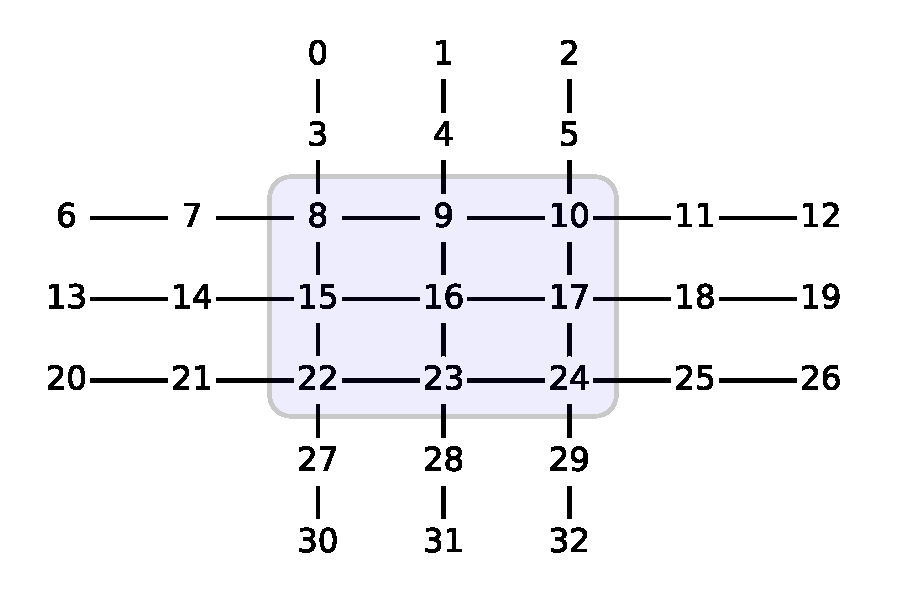
\includegraphics[width=0.29\linewidth]{web1center}
%  }
%  \hfill %\hspace{\figsep}
%  \subcaptionbox{$`a\in [\frac{37}{20},\frac{58}{25}){;}`b = 0.85$\label{fig:2web}}{ %3*9+4*6-12 / 48-9 = 27+12 / 41 = 39/41
%    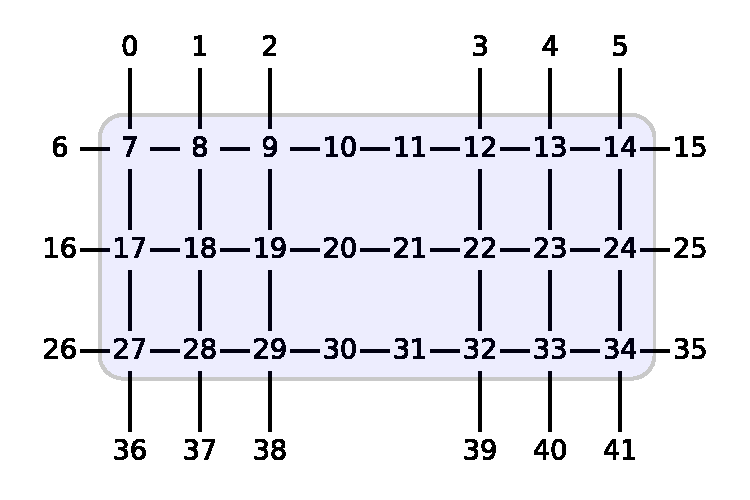
\includegraphics[width=0.3\linewidth]{web2center2}
%  }
%  \hfill %\hspace{\figsep}
%  \subcaptionbox{$`a\in [\frac{58}{25},\frac{75}{32}){;}`b = 0.85$\label{fig:2web2}}{ %3*9+4*6-12 / 48-9 = 27+12 / 41 = 39/41
%    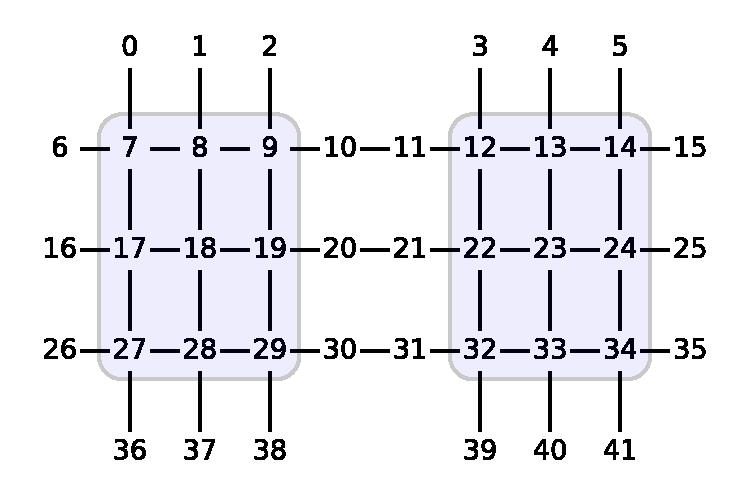
\includegraphics[width=0.3\linewidth]{web2center}
%  }
%  % \hspace{\figsep}
%  % \subcaptionbox{\label{fig:mweb}}{
%    
%  % }
%  \caption{Undirected web graphs with boxes showing web centers identified as $(`a,`b)$-communities for the range of $`a$ and $`b$ specified. There are no other $(`a,`b)$-communities except the entire set of nodes for $`a$ smaller than the specified range.}
%  \label{fig:web-center}
%\end{figure}
%
%\begin{figure}
%  \centering
%  \def\figsep{.4cm}
%  \def\dist{1}
%  \def\disty{.9}
%  \subcaptionbox{$`a\in [\frac{1}{8},\frac1{2})$\label{fig:1web-cc}}{
%    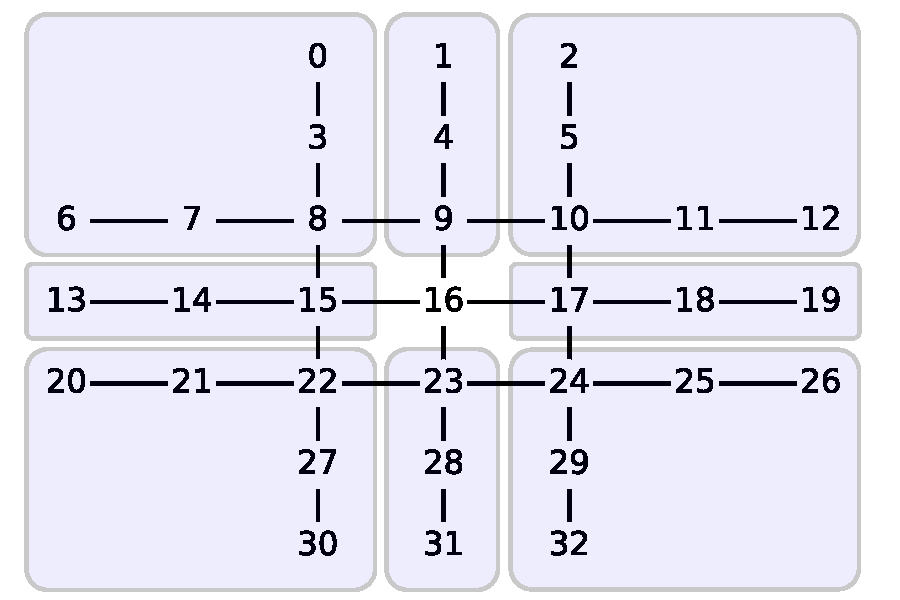
\includegraphics[width=0.3\linewidth]{web1peripheral}
%  }
%  \hfill %\hspace{\figsep}
%  \subcaptionbox{$`a\in [\frac1{2},1)$\label{fig:1web2-cc}}{% 
%    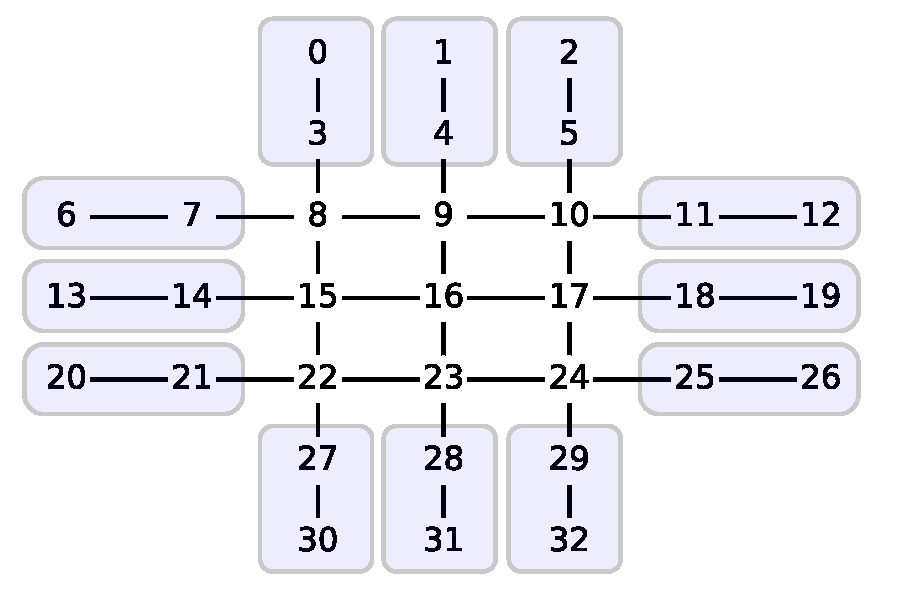
\includegraphics[width=0.3\linewidth]{web1peripheral2}
%  }
%  \hfill %\hspace{\figsep}
%  \subcaptionbox{$`a\in [\frac4{41},1)$\label{fig:2web-cc}}{% 
%    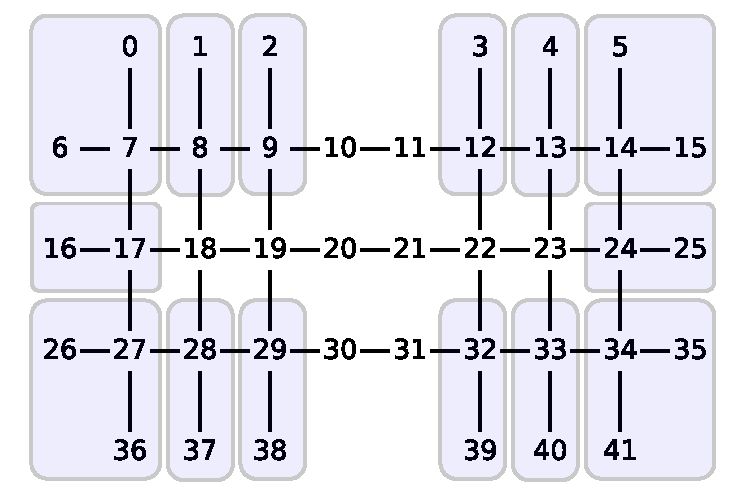
\includegraphics[width=0.3\linewidth]{web2peripheral}
%  }
%  % \hspace{\figsep}
%  % \subcaptionbox{\label{fig:mweb}}{
%    
%  % }
%  \caption{Boxes showing all the communities returned by cut-clustering within the given range of $`a$. The other communities returned are singletons for larger $`a$ and the entire set for smaller $`a$.}
%  \label{fig:web-peripheral}
%\end{figure}


\usetikzlibrary{arrows,patterns}

\pgfdeclarepatternformonly{soft crosshatch}{\pgfqpoint{-1pt}{-1pt}}{\pgfqpoint{4pt}{4pt}}{\pgfqpoint{3pt}{3pt}}%
{
  \pgfsetstrokecolor{blue}
  \pgfsetstrokeopacity{0.3}
  \pgfsetlinewidth{0.4pt}
  \pgfpathmoveto{\pgfqpoint{3.1pt}{0pt}}
  \pgfpathlineto{\pgfqpoint{0pt}{3.1pt}}
  \pgfpathmoveto{\pgfqpoint{0pt}{0pt}}
  \pgfpathlineto{\pgfqpoint{3.1pt}{3.1pt}}
  \pgfusepath{stroke}
}

\tikzstyle{cut}=[fill=red, fill opacity=0.2,rounded corners,inner sep=0.1em]
\tikzstyle{cluster}=[pattern=soft crosshatch, pattern color=blue, fill opacity=0.2,rounded corners,inner sep=0.1em]
\tikzstyle{v}=[circle,draw,fill=gray!40,minimum size=2,transform shape]
\tikzstyle{nodestyle}=[every node/.style={transform shape}]

\begin{figure}
\def\s{.3}
\centering
\subcaptionbox{\label{fig:oneweb-community}}{
\begin{tikzpicture}[scale=\s]
  \foreach \x in {0,...,6}
    \foreach \y in {0,...,2} 
       \node [v]  (a\x\y) at (\x,\y) {};

  \foreach \y in {0,...,2}
    \foreach \x [count=\xi] in {0,...,5}  
      \draw (a\x\y)--(a\xi\y);


  \foreach \x in {0,...,2}
    \foreach \y in {0,...,6} 
       \node [v]  (b\x\y) at (\x+2,\y-2) {};

  \foreach \x in {0,...,2}
    \foreach \y [count=\yi] in {0,...,5}  
      \draw (b\x\y)--(b\x\yi);

	\node[cluster,fit=(a20) (a42)] {};
\end{tikzpicture}
}
%
\subcaptionbox{\label{fig:oneweb-cut1}}{
\begin{tikzpicture}[scale=\s]
  \foreach \x in {0,...,6}
    \foreach \y in {0,...,2} 
       \node [v]  (a\x\y) at (\x,\y) {};

  \foreach \y in {0,...,2}
    \foreach \x [count=\xi] in {0,...,5}  
      \draw (a\x\y)--(a\xi\y);


  \foreach \x in {0,...,2}
    \foreach \y in {0,...,6} 
       \node [v]  (b\x\y) at (\x+2,\y-2) {};

  \foreach \x in {0,...,2}
    \foreach \y [count=\yi] in {0,...,5}  
      \draw (b\x\y)--(b\x\yi);

	\node[cut,fit=(a00) (b00)] {}; \node[cut,fit=(a62) (b26)] {};
	\node[cut,fit=(a02) (b06)] {}; \node[cut,fit=(a60) (b20)] {};
	\node[cut,fit=(a01) (a21)] {}; \node[cut,fit=(a41) (a61)] {};
	\node[cut,fit=(b10) (b12)] {}; \node[cut,fit=(b14) (b16)] {};
\end{tikzpicture}
}
%
\subcaptionbox{\label{fig:oneweb-cut2}}{
\begin{tikzpicture}[scale=\s]
  \foreach \x in {0,...,6}
    \foreach \y in {0,...,2} 
       \node [v]  (a\x\y) at (\x,\y) {};

  \foreach \y in {0,...,2}
    \foreach \x [count=\xi] in {0,...,5}  
      \draw (a\x\y)--(a\xi\y);


  \foreach \x in {0,...,2}
    \foreach \y in {0,...,6} 
       \node [v]  (b\x\y) at (\x+2,\y-2) {};

  \foreach \x in {0,...,2}
    \foreach \y [count=\yi] in {0,...,5}  
      \draw (b\x\y)--(b\x\yi);

	\node[cut,fit=(a00) (a10)] {}; \node[cut,fit=(a50) (a60)] {};
	\node[cut,fit=(a01) (a11)] {}; \node[cut,fit=(a51) (a61)] {};
	\node[cut,fit=(a02) (a12)] {}; \node[cut,fit=(a52) (a62)] {};
	\node[cut,fit=(b00) (b02)] {}; \node[cut,fit=(b04) (b06)] {};
	\node[cut,fit=(b10) (b12)] {}; \node[cut,fit=(b14) (b16)] {};
	\node[cut,fit=(b20) (b22)] {}; \node[cut,fit=(b24) (b26)] {};
\end{tikzpicture}
}
  \caption{
	  An example graph that exhibits a grid-like center that
	  connects to threads of nodes along the grid's perimeter. Communities and cut-clusters are
	  highlighted using a crosshatch (blue) and no-pattern (red) marks, respectively.
	  (a) Shows the returned community for $\alpha \in [\frac{31}{20},\frac{27}{16})$ and $\beta = 0.7$, and 
	  (b) the cut-clusters for $\alpha\in [\frac{1}{8},\frac{1}{2})$
	  and (c) the cut-clusters for $\alpha\in [\frac{1}{2}, 1)$.
	  There are no other non-trivial (i.e., the entire set) solutions.
  }
  \vspace{-1em}
  \label{fig:oneweb}
\end{figure}




\begin{figure}
\def\s{.28}
%\centering
\subcaptionbox{\label{fig:twowebs-community1}}{
\begin{tikzpicture}[scale=\s]
  \foreach \x in {0,...,9}
    \foreach \y in {0,...,2} 
       \node [v]  (a\x\y) at (\x,\y) {};

  \foreach \y in {0,...,2}
    \foreach \x [count=\xi] in {0,...,8}  
      \draw (a\x\y)--(a\xi\y);


  \foreach \x in {0,1,2, 5,6,7}
    \foreach \y in {0,...,4} 
       \node [v]  (b\x\y) at (\x+1,\y-1) {};

  \foreach \x in {0,1,2, 5,6,7}
    \foreach \y [count=\yi] in {0,...,3}  
      \draw (b\x\y)--(b\x\yi);

	\node[cluster,fit=(a10) (a82)] {};
\end{tikzpicture}
}
%
\subcaptionbox{\label{fig:twowebs-community2}}{
\begin{tikzpicture}[scale=\s]
  \foreach \x in {0,...,9}
    \foreach \y in {0,...,2} 
       \node [v]  (a\x\y) at (\x,\y) {};

  \foreach \y in {0,...,2}
    \foreach \x [count=\xi] in {0,...,8}  
      \draw (a\x\y)--(a\xi\y);


  \foreach \x in {0,1,2, 5,6,7}
    \foreach \y in {0,...,4} 
       \node [v]  (b\x\y) at (\x+1,\y-1) {};

  \foreach \x in {0,1,2, 5,6,7}
    \foreach \y [count=\yi] in {0,...,3}  
      \draw (b\x\y)--(b\x\yi);
%
	\node[cluster,fit=(a10) (a32)] {};
	\node[cluster,fit=(a60) (a82)] {};

\end{tikzpicture}
}
%
\subcaptionbox{\label{fig:twowebs-cut}}{
\begin{tikzpicture}[scale=\s]
  \foreach \x in {0,...,9}
    \foreach \y in {0,...,2} 
       \node [v]  (a\x\y) at (\x,\y) {};

  \foreach \y in {0,...,2}
    \foreach \x [count=\xi] in {0,...,8}  
      \draw (a\x\y)--(a\xi\y);


  \foreach \x in {0,1,2, 5,6,7}
    \foreach \y in {0,...,4} 
       \node [v]  (b\x\y) at (\x+1,\y-1) {};

  \foreach \x in {0,1,2, 5,6,7}
    \foreach \y [count=\yi] in {0,...,3}  
      \draw (b\x\y)--(b\x\yi);

	\node[cut,fit=(a00) (b00)] {}; \node[cut,fit=(a92) (b74)] {};
	\node[cut,fit=(a01) (a11)] {}; \node[cut,fit=(a91) (a81)] {};
	\node[cut,fit=(a02) (b04)] {}; \node[cut,fit=(a90) (b70)] {};

	\node[cut,fit=(b10) (b11)] {}; \node[cut,fit=(b13) (b14)] {};
	\node[cut,fit=(b20) (b21)] {}; \node[cut,fit=(b23) (b24)] {};
	\node[cut,fit=(b50) (b51)] {}; \node[cut,fit=(b53) (b54)] {};
	\node[cut,fit=(b60) (b61)] {}; \node[cut,fit=(b63) (b64)] {};
\end{tikzpicture}
}
  \caption{
	  %An example graph that resembles a spider's web in that it exhibits a grid-like center that
	  %connects to threads of nodes along the grid's perimeter.
	  Similar to Fig.~\ref{fig:oneweb}.
	  (a) Shows the returned community for $\alpha \in [\frac{37}{20},\frac{58}{25})$ and $\beta = 0.85$, 
	  (b) the communities for $\alpha\in [\frac{58}{25},\frac{75}{32})$ and $\beta = 0.85$,
	  and (c) the cut-clusters for $\alpha\in [\frac{4}{41}, 1)$.
	  There are no other, non-trivial, solutions.
  }
  \label{fig:twowebs}
\end{figure}


To illustrate the benefits of the proposed communities over cut-clustering for larger networks than
those in \figref{fig:eg12}, we implemented and tested both algorithms on the graphs in
Figs.~\ref{fig:oneweb} and \ref{fig:twowebs}. The graph in \figref{fig:oneweb} contains a grid-like center,
with peripheral-like chains of nodes attached to the grid's perimeter.
The graph in Fig.~\ref{fig:twowebs} is similarly constructed, but with two grid-like centers.
In both figures, it is desirable to differentiate the (denser) grid-like centers from the (sparser)
peripherals.
%centers, i.e., the peripherals of the webs consist of vertex disjoint chains. The goal is to detect
%the web centers as communities since they are the denser subgraphs.


The desired center is identified as a community in Fig.~\ref{fig:oneweb-community}, while
cut-clustering only returns undesirable solutions, Figs.~\ref{fig:oneweb-cut1} and
\ref{fig:oneweb-cut2}. (See the figure's caption for details.) 
Note that the desired center is not a web community since each of its four corner nodes does not
satisfy \eqref{eq:support-community}, which demonstrates the benefit of choosing $\beta > 0$.
This also explains the undesirable behaviour of cut-clustering since a cut-cluster allows at most
one of its members to violate \eqref{eq:support-community} \cite[Lemma~3.1]{flake:cut-clustering}.
(See \ifPAGELIMIT\cite[Appendix~A]{long} \else Appendix~\ref{sec:comparison-cut} \fi for more details.)
Similar observations can be made using Fig.~\ref{fig:twowebs}, where it is not hard to see that the
same issues extend to larger, and other types of, graphs.  More experimental results on synthetic
and real-world data sets can be found in
\ifPAGELIMIT\cite[Appendix~B]{long}.\else Appendix~\ref{sec:comparison-other}.\fi


%To illustrate the benefits of the proposed communities over cut-clustering for larger networks than those in \figref{fig:eg12}, we implemented and tested both algorithms on the graphs in \figref{fig:web-center}. Note that all the graphs in \figref{fig:web-center} contains web centers, each of which consist of nodes interconnected into $2$-by-$2$ grids. The nodes between different web centers, i.e., the peripherals of the webs consist of vertex disjoint chains. The goal is to detect the web centers as communities since they are the denser subgraphs.
%
%As indicated in \figref{fig:web-center}, all web centers are returned as communities when $`a$ and $`b$ are sufficiently large. In contrast, cut-clustering always fail to return the web centers regardless of the choice of $`a$. Instead, the peripherals are returned as shown in \figref{fig:1web-b}, \figref{fig:1web-c}. This is expected because, by \cite[Lemma~3.1]{flake:cut-clustering}, all but one node in a cut cluster must satisfy the condition~\eqref{eq:support-community}. Web centers cannot be cut clusters because their four corner points do not satisfy \eqref{eq:support-community}, e.g., Node 8 in the web center of \figref{fig:1web} and Node 12 in the web center of \figref{fig:2web} has the same number of internal and external edges. The experiments confirm that the internal support plays an important role in identifying the web centers as communities, and so our proposed solution can strictly improves over the previous solution. Following the same logic, it is not difficult to see that the same issue may arise regardless of the number of web centers or how far apart they are. The same problem can also arise in other types of graphs.
%

% Consider the web-spider graph in \figref{fig:web}, which is an undirected graph with edges of unit weight. Cut clustering returns only the four legs and their segments as communities but not the center four more interconnected nodes. (show ...) However, the center is a meaningful community and is returned as an $(`a,`b)$-community for (range of alpha and value of beta).

% \figref{} shows another example where there are more than one web centers. Again, our approach finds the web centers but cut-clustering only returns the leg segments instead of the web centers.

% \figref{} shows another example with more legs and a larger center. Indeed, the center is not a supporting community due to the many external connections to the legs. Again, our approach returns the center but cut-clustering does not. 


\bibliographystyle{IEEEtran}
\bibliography{IEEEabrv,ref}

\ifPAGELIMIT
\else 
\appendices

\section{Comparison with cut-clusters}
\label{sec:comparison-cut}

In this section we compare our formulation to cut-clusters, which were introduced in
\cite{flake:cut-clustering} as a tractable alternative to web-communities.
%Note that when $\beta=0$ and the graph is undirected, the augmented graph in
%Definition~\ref{def:augmented} is the same for all $t\in V$. For this augmented graphs, one can
%compute a Gomory-Hu tree. The cut-clusters are defined as the connected components of the tree after
%deleting the additional node $s$.
%\footnote{
%	aaa--- This is a rough description that ignores some technical issues. Aside from the fact the
%	Gomory-Hu tree is not unique, in \cite{flake:cut-clustering} the community of $t\in V$ w.r.t.
%	$s$ is defined as the inclusion-wise minimum $s$-$t$ cut in the augmented graph. Now while it is
%	argued \cite[Lemma~3.4]{flake:cut-clustering} that for a given $t$ there exists a Gomory-Hu tree
%	that gives this inclusion-wise cut, it is not clear whether there exists a Gomory-Hu that
%	simultaneously satisfy this for all $t \in V$.
%}
%
%Recall Definition~\ref{def:candidates}, the communities in \cite{flake:cut-clustering} are essentially the
%candidates in the special case when the graph is undirected and $`b = 0$.
%More precisely, we have the following proposition.
The following proposition relates the cut-clusters to the candidates of Definition~\ref{def:candidates}.
We start by providing an explicit characterization of cut-clusters, which is absent from 
\cite{flake:cut-clustering}.
\begin{proposition}
  \label{prop:cut-clusters-from-candidates}
  When the graph is undirected and $\beta = 0$, then, for $`a \geq 0$,
  the set of inclusion-wise maximal candidates, with the singletons removed, i.e., 
  \begin{align}
	  \op{maximal} \{C_{`a, t} \mid  t\in V\} \ \backslash \ \{\Set{i} \mid i\in V\},\label{eq:cut-clusters}
  \end{align}
  is equal to the set of cut-clusters returned by the cut-clustering algorithm
  \cite[Fig.~2]{flake:cut-clustering}.
\end{proposition}

\begin{Proof}
  We first define the cut-clusters more precisely as follows.
  Consider an undirected graph and its $`a$-augmented graph in Definition~\ref{def:augmented} but with additional edges $(t,s)$ of weight $`a$ for $t\in V$. Note that the additional edges $(t,s)$ does not contribute to any $s$--$t$ cuts and so all the $s$--$t$ cut values remain unchanged. The purpose of the additional edges is to turn the augmented graph into an undirected augmented graph so that a Gomory-Hu tree of the augmented graph is well-defined. 
  Let $T$ be a Gomory-Hu tree of the undirected augmented graph and $\mcP$ be the set of connected components of $T$ after removing $s$. 
  Recall from \cite{flake:cut-clustering} and the end of Section~\ref{sec:introduction} that the set of cut clusters at threshold $`a$ is the set of non-singleton elements in $\mcP$. Since the Gomory-Hu tree may not be unique, the elements of $\mcP$ are further required to be inclusion-wise minimal. 
  
  We will show that the cut clusters are given by \eqref{eq:cut-clusters}. In particular, we will show that
  \begin{align}
      \mcP\subseteq \op{maximal}\Set{C_{`a,t}\mid t\in V}, \label{eq:cut-clusters:1}
  \end{align}
  which imply the desired result trivially. By the properties of Gomory-Hu tree, for any $t\in V$,
  \begin{enumerate}
      \item\label{prop:cc:1} the $s$--$t$ mincut value $\hat{f}_t(`a)$ of the augmented graph can be obtained as the minimum weight of an edge in the unique path between $s$ and $t$ in $T$, and
      \item\label{prop:cc:2} the connected components of $T$ after removing the minimum weight edge are the cut sets $V`/C$ and $C$ where $C$ is an optimal solution to $\hat{f}_t(`a)$ in \eqref{eq:g-candidate}.
  \end{enumerate}
  For simplicity, consider the case where the solution to $\hat{f}_t(`a)$ in \eqref{eq:g-candidate} is uniquely equal to $C_{`a,t}$ for all $t\in V$. 
  Let $s$ be the root of $T$. It is readily seen that $C_{`a,t}$ corresponds to a proper subtree of $T$ by the above properties. Furthermore, each element of $\mcP$ is equal to $C_{`a,t}$ for a neighbor $t$ of $s$ in $T$, since the path from $s$ to $t$ in $T$ contain only the edge $(s,t)$. This implies \eqref{eq:cut-clusters:1} because $\mcP$ corresponds to the maximal proper subtrees of $T$.
  
  Finally, consider the remaining case where the solution to $\hat{f}_t(`a)$ in \eqref{eq:g-candidate} may not be unique. It suffices to argue that a Gomory-Hu tree exists where the value of $C$ in Property~\ref{prop:cc:2} above is the minimal solution $C_{`a,t}$. We will show that it is possible to increase $`a$ slightly to ensure uniqueness without changing the minimal solutions to $\hat{f}_t(`a)$. More precisely, let $\mcC_{`a,t}$ be the set of solutions to $\hat{f}_t(`a)$. Consider any $`a'>`a$. Since $f_{`a}(C)$ is increasing in $`a$ and $C$,
  \[C\not\in \mcC_{`a',t}\quad \forall t\in V, C\in \mcC_{`a,t}`/\Set{C_{`a,t}}.\]
  However, since $f_{`a}(C)$ is continuous in $`a$, it is possible to choose $`a'$ sufficiently close to $`a$ such that
  \[ \mcC_{`a',t} = \Set{C_{`a,t}} \quad \forall t\in V,\] 
  i.e., $C_{`a,t}$ remains optimal and not other $s$--$t$ cuts become optimal as we goes from $`a$ to $`a'$. Any Gomory-Hu tree of the $`a'$-augmented graph with edge weight $\hat{f}_t(`a')$ replaced by $\hat{f}_t(`a)$ satisfy Property~\ref{prop:cc:1} and \ref{prop:cc:2}. Hence, it can be used as the desired Gomory-Hu tree.
\end{Proof}


% %
% %%Proof by construct the tree.
% \textcolor{blue}{[old, to be deleted]\\
% Proof: Denote maximal$\{C_{\alpha 0 t}\}=\{C_1, C_2, \dots, C_m\}$, and denote a dominant node in $C_i$ as ${b_i}$, s.t. $C_i$ is the minimal solution for $\hat{f}_{b_i}(\alpha), i=1,2,...,m$.\\
% Introduce an artificial node $a$ with edges of weight $\alpha$ connecting to every node in V. 
% Then for each $i=1,2,...,m$, choose the Gomory-Hu tree between node $a$ and $b_i$ s.t. cutting the edge between $a$ and $b_i$ in the tree will separate cluster $C_i$, and this is achievable according to Definition \ref{def:augmented} and Theorem \ref{thm:mc}, and the weight of edge between $a$ and $b_i$ is $\hat{f}_{b_i}(\alpha)$. Cut the edges between $a$ and $b_i$ in the tree, and denote the obtained branch containing $b_i$ as $B^i$.\\
% From Theorem \ref{thm:hierarchy} we can know that $C_i \cap C_j = \emptyset, \forall 1 \leq i,j \leq m, i \neq j$. Hence, we can connect each branch $B^i, i=1,2,...,m,$ that obtained in the last step to the artificial node $a$ with weight $\hat{f}_{b_i}(\alpha)$. It is easy to verify that the new tree is a Gomory-Hu tree for all the nodes appear in maximal$\{C_{\alpha 0 t}\}$. Then, remove the node $a$, we will obtain the cut-clusters.\\
% }
% \\%%%%%
% Proof: Denote maximal$\{C_{\alpha 0 t} | t \in V \}=\{C_1, C_2, \dots, C_m\}$, then every node in V will appear in maximal$\{C_{\alpha 0 t} | t \in V \}$. Denote a dominant node in $C_i$ as ${b_i}$, s.t. $C_i$ is the minimal solution for $\hat{f}_{b_i}(\alpha), i=1,2,...,m$.\\
% Introduce an artificial node $a$ with edges of weight $\alpha$ connecting to every node in V, and this will be the same augmented graph with the augmented graph in Definition \ref{def:augmented}.\\
% For each $i=1,2,...,m$, choose the Gomory-Hu tree containing an edge between node $a$ and $b_i$ s.t. cutting the edge between $a$ and $b_i$ in the tree will separate cluster $C_i$, and this is achievable according to the existence of Gomory-Hu tree and the construction method of Gomory-Hu tree. Then the mincut between $a$ and nodes in $C_i$ (including $b_i$) is the weight of edge between $a$ and $b_i$ in the tree, and the edge possesses the smallest weight aomong edges between $\{a\} \cup C_i$ in the Gomory-Hu tree.\\ 
% Since the graph after adding the node $a$ and corresponding edges here is the same as the augmented graph in Definition \ref{def:augmented}, according to Theorem \ref{thm:mc}, the weight of edge between $a$ and $b_i$ in the selected Gomory-Hu tree is $\hat{f}_{b_i}(\alpha)$. Cut the edges between $a$ and $b_i$ in the tree, and denote the branch that containing $b_i$ as $B^i$, In the branch $B^i$, the Gomory-Hu tree structure for nodes in $B^i$ is reserved (if $C_i=\{b_i\}, 1 \leq i \leq m$, is a singleton set, then the branch is the node $b_i$ itself).\\
% Connect each branch $B^i, i=1,2,...,m,$ that obtained and in the last step to the artificial node $a$ by adding an edge with weight $\hat{f}_{b_i}(\alpha)$ between $a$ and $b_i$, considering Theorem \ref{thm:hierarchy} we can know that $C_i \cap C_j = \emptyset, \forall 1 \leq i,j \leq m, i \neq j$, so each node from V will only appear once.\\ 
% By checking the mincut between nodes inside the same $C_i$ (the mincut is the smallest edge in the path between the two nodes in the branch $B^i$), and the mincut between $a$ and nodes in $C_i$ (the mincut is $\hat{f}_{b_i}(\alpha)$, which is the weight of edge between $a$ and $b_i$ in the tree, and we have known edge between $a$ and $b_i$ is edge with the smallest weight among the edges in $\{a\} \cup C_i$ in the tree), and the mincut between nodes between $C_i$ and $C_j$ (the mincut is $min\{\hat{f}_{b_i}(\alpha), \hat{f}_{b_j}(\alpha)$ \}, and considering that the path between any two node in the tree is unique, we can know that the mincut between any two nodes can be represent by the weight of the smallest edge of the unique path in the tree between the two nodes. So the new tree is a Gomory-Hu tree for the augmented graph.\\ 
% So the constructed Gomory-Hu tree can be used as the tree for obtaining cut-clusters by removing the node $a$, and then the clusters $C_1, C_2,...,C_m$ are obtained, and the clusters with size larger than 1 are cut-clusters, which can be represented as $\{C_i | 1 \leq i \leq m, |C_i|>1 \}$, or maximal$\{C_{\alpha 0 t} | t \in V \} \setminus \{\{i\} | i \in V \}$.\\

%%%%%%%%%%%%%%
\begin{example}
	\label{eg:chain-cut}
	Consider the undirected graph in Fig.~\ref{fig:eg-chain}.
	The webcommunities are listed in \eqref{eq:chain-communities}.
%
	Proposition~\ref{prop:cut-clusters-from-candidates} asserts that the cut-clusters are specified
	by $\hat{f}_{t}(\alpha)$ for $t\in V$ (solid curves) in Fig.~\ref{fig:eg-chain-beta0} as
	\begin{align}
			\label{eq:eg-chain-cut}
			\left\{
				\!\!\!
				\begin{array}{l@{\ }l}
					%\Set{0}, \Set{1}, \Set{2}, \Set{3}, & `a \geq 2  
					\emptyset, & `a \geq 2  
					\\
					\Set{0,1}, \Set{2,3}, & `a \in [1.5, 2)
					\\
					\Set{0,1,2,3}, &  `a < 1.5 \ ,
				\end{array}
			\right.
	\end{align}
	i.e., they are obtained by choosing the maximal elements in each row of \eqref{eq:eg-chain-candidates}.
	Note that, in contrast to communities at $\beta = 0$, a cut-cluster may 
	not be web-community, e.g., for the cut-cluster $\Set{0,1}$, node $1$  has more
	connections with the external node $2$ than it has with the member node $0$.
	This contrast between cut-clusters and communities at $\beta = 0$
	can be seen by comparing \eqref{eq:single-shrink} and \cite[Lemma~3.1]{flake:cut-clustering}.
	Namely, while \eqref{eq:single-shrink} guarantees a positive gap between the internal and external
	influences for every member of the community, \cite[Lemma~3.1]{flake:cut-clustering} guarantees this
	for every member of the cut-cluster except possibly one member. 
	%
	Finally, note that cut-clustering fails to find the web-community $\Set{1,2}$ since the formulation
	lacks the ability to reward internal connections, see Example~\ref{eg:chain-community}.
\end{example}
%%%%%%%%%%%%%

%
	In addition to their closer relation to web-communities (as observed in the previous example) communities at
	$\beta = 0$ 
	%Although both the communities at $\beta=0$ and the cut-clusters are obtained from the candidates
	%at $\beta=0$, it is important to note that the communities
	also come with stronger quality guarantees compared to cut-clusters.  This follows by observing that \eqref{eq:bound-beta0}~\uref{ii}
provides a stronger guarantee than the bound on the expansion in \cite[Theorem~3.3]{flake:cut-clustering} 
\begin{align}
  `a \leq \min_{B\subsetneq C: \abs{B}\geq 1} \frac{w(C`/B,B)}{\min\Set{\abs{C`/B},\abs{B}}}. \label{eq:expand}
\end{align}
More precisely, for undirected graphs, \eqref{eq:bound-beta0}~\uref{ii} implies
\begin{align}
  \begin{split}
  `a &< \min_{B\subsetneq C: \abs{B}\geq 1} \Set*{\frac{w(C`/B,B)}{\abs{C`/B}}, \frac{w(B,C`/B)}{\abs{B}}}\\
  &= \min_{B\subsetneq C: \abs{B}\geq 1} \frac{w(C`/B,B)}{\max\Set{\abs{C`/B},\abs{B}}}.
  \end{split}
  \label{eq:expand_improved}
\end{align}
This is the same as \eqref{eq:expand} except that the minimization in the denominator is replaced by
maximization, which gives a potentially better bound.

\textcolor{magenta}{
	aaa---possibly connect the above paragraph to conductance comparison.
}



%{\color{magenta} 
Finally, in contrast to Theorem~\ref{thm:hierarchy} which can be extended to a general submodular function,
the hierarchical structure for cut-clusters in \cite[Lemma~3.9]{flake:cut-clustering} relies on the specific
formulation using the undirected graph cut. In particular, the result does not extend to digraphs
where the incut function is not symmetric. For instance, consider the digraph in 
Fig.~\ref{fig:eg-dchain}, which can be obtained from the graph in \figref{fig:eg-chain}
by setting $w(0,1)=w(3,2)=0$.
%instead of $2$. We still have
%$w(1,0)=w(2,3)=2$, i.e., we remove the outgoing edges of $0$ and $3$ but not the incoming edges.
With $`a\in [0,1)$ and $`b=0$, it can be shown that $C_{`a,t}$ for $t=0$ and $3$ are
$\Set{0,1,2}$ and $\Set{1,2,3}$ respectively, which are neither disjoint nor subsets of each
other.
%}



%{\color{magenta}
%Move to comparison from formulation:
%Note that the requirement for a community to be both minimal and non-singleton among all solutions
%of~\eqref{eq:alpha-beta-community} is more stringent than simply imposing $\abs{C}>1$ in
%\eqref{eq:alpha-beta-community} or requiring the community to be minimal among all non-singleton
%solutions. In particular, a community satisfying such requirement may not exist for some choices of
%$(`a,`b)$. This more stringent requirement was not considered in \cite{flake:cut-clustering}.
%However, instead of limiting the usefulness of the definition, the requirement leads to the
%following stronger guarantee on the quality of community than
%\cite[Lemma~3.1]{flake:cut-clustering}. 
%}



%\textcolor{magenta}{
%As illustrated by the following example, our approach not only provides an extension of
%cut-clustering to digraphs, but can also improve the quality of the returned communities for
%undirected graphs.
%}




%\begin{example}
%	\label{eg:chain}
%	Consider the undirected graph in Fig.~\ref{fig:eg-chain}. It is straightforward to enumerate all the
%	supporting communities \eqref{eq:support-community} as
%	$
%	\Set{0,1,2,3},
%	\Set{0,1,2},
%	\Set{1,2,3}, %\text{and}
%	\Set{1,2}.
%	$
%%	It can also be shown that the cut-clusters \cite[Fig.~2]{flake:cut-clusteing} are 
%%	\begin{align}
%%		\left\{
%%			\begin{array}{ll}
%%				\Set{0,1,2,3}, &  `a < 1.5 \\
%%				\Set{0,1}, \Set{2,3}, & `a \in [1.5, 2) \\
%%				\Set{0}, \Set{1}, \Set{2}, \Set{3}, & `a \geq 2, 
%%			\end{array}
%%		\right.
%%	\end{align}
%%	while the $(`a,0)$-communities are
%%	\begin{align}
%%		\left\{
%%			\begin{array}{ll}
%%				\Set{0,1,2,3}, & `a < 2/3 \\
%%				\text{none}, & `a \geq  2/3 
%%			\end{array}
%%		\right.
%%	\end{align}
%%	and the $(`a,1)$-communities are
%%	\begin{align}
%%		\left\{
%%			\begin{array}{ll}
%%				\Set{0,1,2,3}, & `a < 2/3 \\
%%				\Set{1,2}, & `a \in  [2/3, 3) \\
%%				\text{none}, & `a \geq 3
%%			\end{array}
%%		\right.
%%	\end{align}
%	%It can also be shown that the cut-clusters \cite[Fig.~2]{flake:cut-clustering}, $(`a,0)$-communities, and $(`a,1)$-communities are as follows.
%	To compute the $(`a,`b)$-communities, and cut-clusters we apply
%	Propositions~\ref{prop:communities-from-candidates} and \ref{prop:cut-clusters-from-candidates},
%	respectively. For $`b = 0$ and $1$, respectively,
%	Figs.~\ref{fig:eg-chain-beta0} and \ref{fig:eg-chain-beta1} show the plots (against $`a$) of the functions $g(`a,`b)$
%	(blue, see \eqref{eq:alpha-beta-community} or \eqref{eq:g-community}), $g_{t}(`a,`b)$
%	(solid black, see \eqref{eq:g-candidate}), and
%	%$f_{`b}(C_{`a`bt}) + `a\ccdot |C_{`a`bt}|$ (dashed black).
%	$f_{\alpha\beta}(C)$ (dashed black).%
%	\footnote{
%	The figure shows $f_{\alpha\beta}(C)$ only for the relevant
%	subsets $C\subseteq V$ achieving \eqref{eq:g-candidate}, i.e., the $(\alpha,\beta)$-candidates. In
%	other words, all suppressed lines lie above the curve of $g_{t}$ for all $t\in V$.
%	}
%	The cut-clusters can be read out from $g_{t}(\alpha,0)$ for $t\in V$ (solid curves) in Fig.~\ref{fig:eg-chain-beta0}
%	as
%	\begin{align}
%			\left\{
%				\!\!\!
%				\begin{array}{l@{\ }l}
%					\Set{0}, \Set{1}, \Set{2}, \Set{3}, & `a \geq 2  
%					\\
%					\Set{0,1}, \Set{2,3}, & `a \in [1.5, 2)
%					\\
%					\Set{0,1,2,3}, &  `a < 1.5
%				\end{array}\!\!,
%			\right.
%	\end{align}
%	and the $(\alpha,\beta)$-communities, for $\beta=0$ and $1$, can be read out from
%	$g(\alpha,\beta)$ (blue solid curves) in Figs.~\ref{fig:eg-chain-beta0} and
%	\ref{fig:eg-chain-beta1} as
%	\begin{align}
%		\label{eq:eg-chain}
%		\begin{array}{c@{\,\,}c}
%			 (`a,0)\text{-communities} & (`a,1)\text{-communities} \\[\smallskipamount]
%			\!\!
%			\!\!
%			\left\{
%				\!\!\!
%				\begin{array}{l@{\ }l}
%					\emptyset, & `a \geq  2/3 
%					\\
%					\Set{0,1,2,3}, & `a < 2/3
%				\end{array}\!\!,
%			\right.
%			&
%			\left\{
%				\!\!\!
%				\begin{array}{l@{\ }l}
%					\emptyset, & `a \geq 6
%					\\
%					\Set{1,2}, & `a \in  [4, 6)
%					\\
%					\Set{0,1,2,3}, & `a < 4
%				\end{array}\!\!.
%			\right.
%		\end{array}
%	\end{align}
%Note that, except for the trivial community $\Set{0,1,2,3}$, none of the cut-clusters
%is a supporting community, e.g., for the cut-clustering community $\Set{0,1}$, node $1$  has more
%connections with the external node $2$ than it has with the community member node $0$.
%%In contrast, all the $(`a,0)$ and $(`a,1)$-communities in this example are supporting
%%communities.  \textcolor{brown}{ (This is not true in general for $`b > 0$, see \eqref{eq:single-shrink}.) }
%In contrast, all the $(`a,0)$-communities (trivial in this example) are supporting communities,
%%see Theorem~\ref{theorem:single-deviation}.
%see Corollary~\ref{cor:alpha-beta-supporting}.
%
%Another interesting observation is that the supporting community $\Set{1,2}$, which is absent from
%the cut-clustering solution, is captured when
%$`b = 1$, i.e., when the cost function \eqref{eq:fb} rewards the
%internal support.
%%This shows the benefit of choosing $`b > 0$, and the
%%limitation of the cut-clustering algorithm that it ignores the large
%%internal of $\Set{1,2}$.
%This situation may persist in general, and shows the benefit of choosing $\beta > 0$, since a dense subgraph may exhibit strong external connections with the
%rest of the graph compared to the external connections of a sparser subgraph. In this situation, it is intuitive
%to regard the dense subgraph, rather than the sparse one, as a community as long as the external connections of this dense subgraph are weak compared to its 
%internal ones.
%
%% Finally, we remark that although in general an $(`a,`b)$-community for $`b > 0$ might not be a supporting
%% community, such a community can still be desirable as argued in \textcolor{brown}{aaa---add links to
%% relevant discussions / example.} In this context, it is hard to justify the cut-clustering
%% communities $\Set{1,2}$ and $\Set{2,3}$, which appear to be meaningless. 
%
%% \textcolor{brown}{aaa---possibly explain why $\Set{0,1}$ and $\Set{2,3}$ are cut-clusters and not
%% $(`a,0)$-communities. }
%
%
%% %Note that the most interesting supporting community in this example $\Set{1,2}$ is absent from
%% %the cut-clustering and the $`b=0$ solutions, but is captured when
%% %$`b = 1$, i.e., when the cost function \eqref{eq:f-cost} focusses on the internal support instead of the
%% %external support. This shows the benefit of choosing $`b > 0$ in general where one may need to pay
%% %some attention to the internal support in addition to external support.
%% %
%% %Note that, except for the trivial community $\Set{0,1,2,3}$, none of the cut-clusters
%% %is a supporting community, e.g., for the cut-cluster $\Set{0,1}$, node $1$  has more
%% %connections with the external node $2$ than it has with the community member node $0$.
%% %%In contrast, all the $(`a,0)$ and $(`a,1)$-communities in this example are supporting
%% %%communities.  \textcolor{brown}{ (This is not true in general for $`b > 0$, see \eqref{eq:single-shrink}.) }
%% %In contrast, all the $(`a,0)$-communities (trivial in this example) are supporting communities,
%% %%see Theorem~\ref{theorem:single-deviation}.
%% %see Corollary~\ref{cor:alpha-beta-supporting}.
%
%
%% \textcolor{brown}{aaa---move the following paragraph somewhere else, but still can point out
%% 	Figs.~\ref{fig:eg-chain-beta0} and \ref{fig:eg-chain-beta1} for illustration.}
%
%% Note that the functions $f_{`b}(C) + `a\ccdot
%% |C|$, for $C\subseteq V:|C|\geq 1$ are linear in $`a$ with integer slopes from
%% $\Set{1,\dots,n}$. Consequently, the functions $g_{t}(`a,`b)$ and $g(`a,`b)$ are
%% piecewise linear with at most $n$ line segments each and $n-1$ turning points.
%% \textcolor{brown}{possibly comment / link the above discussion to the computation section.}
%\end{example}


\section{comparison with other formulations}
\label{sec:comparison-other}

In this section we compare our formulation to some existing ones. To simplify the discussions, we
rely on simple examples to demonstrate some of the common issues that arise in graph clustering, and
to point out similarities / differences between our method and some existing ones. We also present
some experimental results on synthetic and real-world data sets to verify that our observatoins
extend beyond demonstrating examples.

%\textcolor{magenta}{aaa---this section is still under construction. in the short paper, the section will be replaced by
%a paragraph in the previous section or a pointer.}
%most relevant works are that of Flake et al. \cite{flake:cut-clustering} and
%that of Nagano et al. \cite{nagano2011size}.  We also point out some issues
%that are known to be  problematic for some common clustering techniques, such
%as modularity \cite{newman2006modularity}, Infomap \cite{rosvall2009map}, and
%conductance \cite{add} minimization, but are circumvented in the current
%formulation.


% k-densest sub-graph
The work of \cite{nagano2011size} uses the idea of principle
sequence~\cite{fujishige80,fujishige05,fujishige-pp-revisited} to give a polynomial-time partial
solution to the NP-hard size-constrained submodular function minimization problem. When applied to
graphical networks, the problem reduces to the densest $k$-subgraph problem, and the proposed
solution can be used to identify a portions of the densest $k$-subgraphs.
%Same as the minimum
%average cost clustering, the method in full generality does not have a precise interpretation in
%specific domains. It is different from our framework, as results in \figref{fig:cnr-2000} show that
%our approach can identify strictly more densest subgraphs.
%
%The work in \cite{nagano2011size} considered the size-constrained minimization problem of a
%submodular function.  To make the comparison more concrete (and brief), we focus on the densest
%subgraph problem. The problem is hard in general, however, as shown in \cite{nagano2011size}, 
%it can be partially solved (i.e., for a subset of sizes) using the same formulation
%\eqref{eq:fhat}--\eqref{eq:fb}
In this case the formulation  in \cite{nagano2011size} is similar to 
\eqref{eq:alpha-beta-community} 
with $\beta = 1$ and the constraint $|C| \geq 1$
absent from \eqref{eq:fhat}, i.e., we exclude the empty
set and \cite{nagano2011size} does not.
%. The difference between the
%\eqref{eq:fab}, i.e., it did not exclude the empty set.
It can be shown that this exclusion allows our formulation to fined more solutions to the densest
$k$-subgraph problem. For instance, 
in the graph in Fig.~\ref{fig:eg-chain}, the densest $2$-subgraph is $\Set{1,2}$, which can be
obtained using our algorithm with $\beta = 1$ and $\alpha \in [4,6)$, see
Example~\ref{eg:chain-community}, but cannot be obtained using the formulation in
\cite{nagano2011size} since the empty set achieves a minimum cost of zero over that range of
$\alpha$.
For the same reason the formulation in \cite{nagano2011size} cannot find any community when
$f$ is chosen to be the in-cut function, i.e., $\beta = 0$, since the empty set is trivially the
optimal solution with zero size and zero in-cut.

%%%%%%%%%%%%%% figure: cnr2000
\begin{figure}[h!]
  \vspace{-1em}
  \centering
  \def\figsep{.2cm}
  \def\dist{1}
  \def\disty{.9}
  \begin{subfigure}[b]{.24\textwidth}
    \subcaptionbox{Our approach with $\beta = 1$ \label{fig:cnr-2000-ab}}{%
      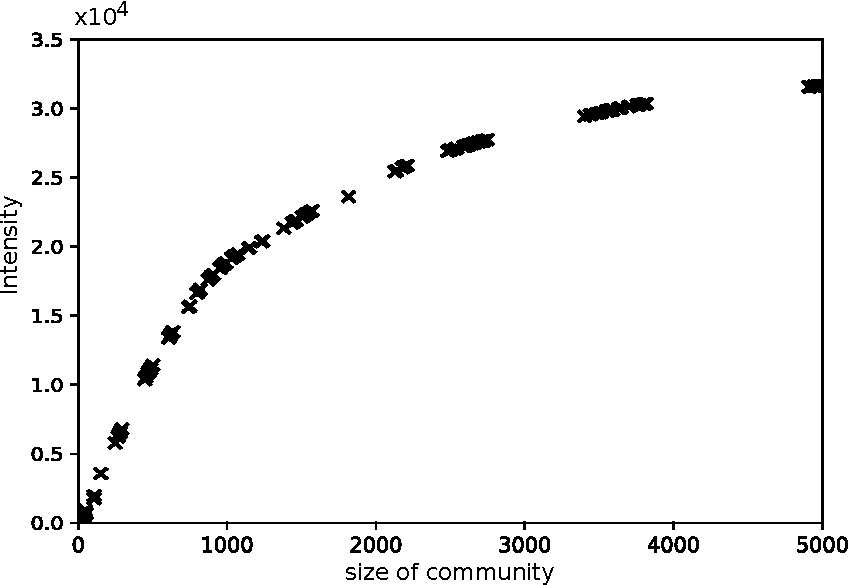
\includegraphics[width=\linewidth]{ab_cnr-2000.pdf}
    }
    % \label{fig:cnr-2000-ab}    
  \end{subfigure}
  \hfill
  \begin{subfigure}[b]{.24\textwidth}
    \subcaptionbox{SSM algorithm. (\cite{nagano2011size})\label{fig:cnr-2000-nagano}}{%
      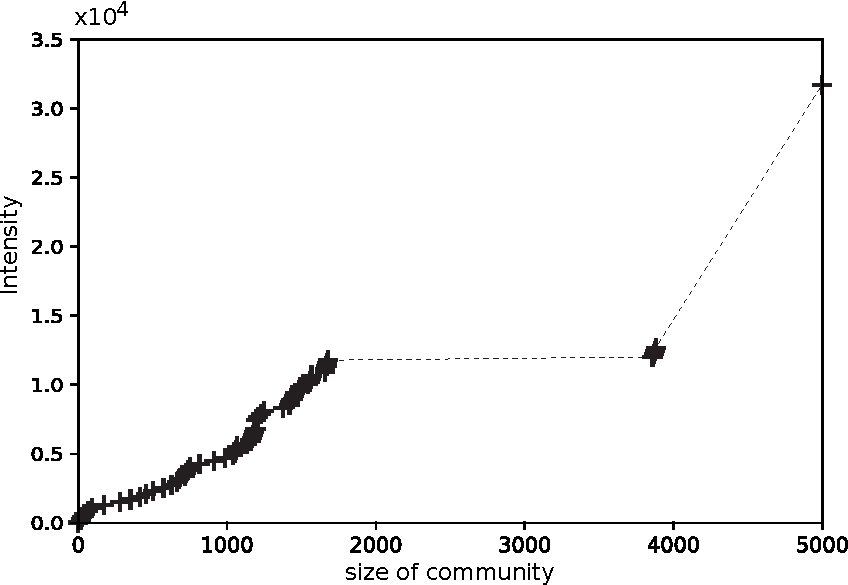
\includegraphics[width=\linewidth]{nagano_cnr-2000.pdf}
    }
    % \label{fig:cnr-2000-nagano}    
  \end{subfigure}
  \caption{Intensity (i.e., total weight of internal edges) versus the size (number of vertices) of
	  the subgraphs returned by (a) our approach and (b) by \cite{nagano2011size}.
	  %Our formulation returns more solutions (densest $k$-subgraphs) than 
	  %plots showing that the proposed algorithm discovers more densest subgraphts of
	  %large sizes. Our method retrieves 51 dense communities with cardinality $>$ 2000 while
	  %the SSM algorithm in \cite{nagano2011size} only finds 2 such communities.}
  }
  \label{fig:cnr-2000}
\end{figure}

%%%%%%%%%%%%%% figure: cnr2000
The observation above extends to larger graphs, which is demonstrated in Fig.~\ref{fig:cnr-2000}.
In this experiment, we applied our algorithm with $\beta = 1$ to the social-network data set
\emph{cnr-2000}, which is a directed unweighted graph. We preprocessed the network in the same way
as \cite{nagano2011size}.
By comparing the result of our algorithm to their proposed SSM algorithm, we are able to retrieve
$51$ dense communities with cardinality larger than $2000$, while \cite{nagano2011size} reported that their SSM algorithm can only find
two such communities.

We pause here and remark that a web community is not necessarily a densest subgraph.\footnote{Not to be confused
	with our discussion in an earlier section where we remarked that a densest subgraph is not necessarily a web community, e.g., see
	Fig.~\ref{fig:eg-star}.} 
For instance, consider the graph in Fig.~\ref{fig:DSP}.  The set $\{0,1\}$ is a web community
that is returned by our method, but it is not a densest $2$-subgraph since the subgraph $\{2,3\}$
has strictly more internal connections.  Hence, any graph clustering algorithm that only returns densest
subgraphs will fail to return such a web community.


The modularity \cite{newman2006modularity}, Infomap \cite{rosvall2009map}, and conductance
minimization \cite{shi2000normalized} formulations lead to NP-hard problems, and so rely on
approximations.
Modularity optimization, despite its popularity, has some limitations as pointed out in
\cite{fortunato2007resolution}. One limitation is the resolution limit where the modularity score tends to favour larger
communities. 
For instance, for the graph in Fig.~\ref{fig:modularity_2} (left), the  modularity score is
minimized by the entire set, and so it fails to detect the more meaningful communities $\Set{0,1}$
and $\Set{2,3}$, which can be identified using our formulation.
Another example is  the ring of cliques \cite{fortunato2007resolution} shown in \ref{fig:modularity_2} (right) for 
$30$ cliques each of size $5$. In this case, the modularity method
groups two consecutive cliques as one cluster, while our formulation can identify every clique.
%
Methods that are based on conductance minimization may also suffer since they tend to favour solutions of
%Conductance-minimization based methods may also suffer since they tend to favour solutions of
relatively equal size.\footnote{While this is desirable in some applications, it can also lead to some
undesirable solutions.} An example graph demonstrating this is shown in Fig.~\ref{fig:conductance}.
A similiar issue is faced by Infomap as shown in Figs.~\ref{fig:infomap} and \ref{fig:infomap2}.


Finally, Fig. \ref{fig:LFR} shows that many existing methods fail to find strong communities
\eqref{eq:`s} of large sizes as compared to our method. (See the figure's caption for details.)
The experiment was conducted on a random graph generated according to the LFR benchmark with $\mu = 0.1$
\cite{lancichinetti2009benchmarks}.
%result uses a synthetic graphical network randomly generated using an existing method.
However, the LFR model generates graphs that are geared towards partitional clustering methods,
and so we expect even more discrepancies when testing on real-world networks that are hierarchical
in nature.
%It is also an interesting but challenging problem to generate synethetic networks to test hierarchical clustering methods.


%%%%%%%%%%%% figure: small graphs
\tikzstyle{cluster}=[fill opacity=0.2,rounded corners,inner sep=0.1em]

\begin{figure}[t]
  \centering
  \tikzstyle{nodestyle}=[inner sep=0.2em,outer sep=0em]
  \tikzstyle{every to}=[every node/.style={font=\scriptsize}]
  \begin{subfigure}[b]{.45\textwidth}
    \centering
    \begin{tikzpicture}
      \matrix (DSP) [matrix of math nodes,column sep=1.2em, row sep=1em, nodes={nodestyle}]
      {
	|(0)| 0 & |(1)| 1 & |(2)| 2 & |(3)| 3 & |(4)| 4 \\
      };
      \draw (0) to node [above] {1} (1) (2) to node [above] {2} (3) to node [above] {1} (4);
      \node[cluster,fill=blue,fit=(0) (1)] {};
      \node[cluster,draw=red,fit=(2) (3)] {};
    \end{tikzpicture}
    \caption{Densest subgraphs: The set $\{0,1\}$ is a web-community that is not a densest $2$-subgraph since $\{2,3\}$ has strictly more internal support.}
    \label{fig:DSP}    
  \end{subfigure}
  %%%%%%%%%%%%%%%
  \hfill
  %%%%%%%%%%%%%%%
  \begin{subfigure}[b]{0.45\textwidth}
    % for drawing ring of clique
    % https://tex.stackexchange.com/questions/223854/drawing-a-ring-of-cliques-in-tikz-graphs/223902#223902
    \newcommand\single[2]{ % #1=labels, #2= n=number of nodes
      \foreach \x in {1,...,#2}{
        \pgfmathsetmacro{\ang}{360/#2}
        \pgfmathparse{(\x-1)*\ang}
        \node[draw,fill=red,circle,inner sep=1pt] (#1-\x) at (\pgfmathresult:4cm) {};
      }
      \foreach \x [count=\xi from 1] in {1,...,#2}{
        \foreach \y in {\x,...,#2}{
          \path (#1-\xi) edge[-] (#1-\y);
        }
      }
    }
    \centering
    \begin{tikzpicture}
    \begin{scope}[local bounding box=scope1]
    %\node at (0,0){$n=5, m=30$};
    \node at (0,0){$30$ cliques};
    \end{scope}
    \foreach \s[count=\si from 0] in {0,45,90,...,360}{
    \begin{scope}[shift={($(scope1) +(\s:2)$)}, scale=0.1,rotate=\s+90]
    \single{\si}{5};
    \end{scope}
    }
    \foreach \i/\j in {1/2,2/3,3/4,4/5,5/6,6/7,7/8}
    \draw (\i-1)--(\j-3);
    %\draw[dotted,thick, outer sep=10pt] (8-1)--(1-3);
	 \def\dd{.13cm}
    \draw[dotted,thick, outer sep=10pt] ([xshift=-\dd, yshift=\dd]8-1.north)--([xshift=\dd, yshift=-\dd]1-3.south);
    \end{tikzpicture}
	 %
	 \hfill
    \begin{tikzpicture}
      \matrix (DSP) [matrix of math nodes,column sep=1.9em, row sep=2em, nodes={nodestyle}]
      {
		|(0)| 0 \\ |(1)| 1 \\ |(2)| 2 \\ |(3)| 3 \\
      };
		\draw (0) to node [left] {1} (1) (1) to node [left, rotate=0] {$0.6$} (2) to node [left] {1} (3);
      \node[cluster,inner sep=.3em,fill=blue,fit=(0) (1)] {};
      \node[cluster,inner sep=.3em,fill=blue,fit=(2) (3)] {};
      \node[cluster,inner sep=.9em, draw=red,fit=(0) (3)] {};
    \end{tikzpicture}
    \caption{Modularity: Two graphs showing modularity's bias towards solutions of larger size.}
    \label{fig:modularity_2}
  \end{subfigure}
  %%%%%%%%%%%%%%%
  \hfill
  %%%%%%%%%%%%%%%
  \begin{subfigure}[b]{.45\textwidth}
    \centering
    \begin{tikzpicture}
      \matrix (con) [matrix of math nodes,column sep=1.2em, row sep=1em, nodes={nodestyle}]
      {
		|(0)| 0 & |(1)| 1 & |(2)| 2 & |(3)| 3 & |(4)| 4 & |(5)| 5 & |(6)| 6 & |(7)| 7 & |(8)| 8 & |(9)| 9\\
      };
      \draw (0) to node [above] {2} (1) to node [above] {0.6} (2) to node [above] {1} (3) to node [above] {1} (4) to node [above] {1} (5) to node [above] {1} (6) to node [above] {1} (7) to node [above] {1} (8) to node [above] {1} (9);
      \node[cluster,fill=blue,fit=(0) (1)] {};
      \node[cluster,draw=red,fit=(0) (1) (2) (3) (4),inner sep=0.4em] {};
      %\node[cluster,draw=red,fit=(5) (6) (7) (8) (9),inner sep=0.4em] {};
    \end{tikzpicture}
    \caption{Minimum conductance: The sets $\{0,1,2,3,4\}$ and $\{5,6,7,8,9\}$ minimize the conductance to $\frac19$. In contrast,
our approach can return the desired cluster
$\{0,1\}$.}
    \label{fig:conductance}    
  \end{subfigure}
  %%%%%%%%%%%%%%%
  \hfill
  %%%%%%%%%%%%%%%
  \begin{minipage}[b]{0.45\textwidth}
  \begin{subfigure}[b]{\textwidth}
    \centering
    \begin{tikzpicture}
      \matrix (con) [matrix of math nodes,column sep=1.2em, row sep=1em, nodes={nodestyle}]
      {
		|(0)| 0 & |(1)| 1 & |(2)| 2 & |(3)| 3 & |(4)| 4 & |(5)| 5 & |(6)| 6 & |(7)| 7 & |(8)| 8 & |(9)| 9\\
      };
      \draw (0) to node [above] {2} (1) to node [above] {0.6} (2) to node [above] {1} (3) to node [above] {1} (4) to node [above] {1} (5) to node [right] {1} (6) to node [above] {1} (7) to node [above] {1} (8) to node [above] {1} (9);
      \node[cluster,fill=blue,fit=(2) (3) (4) (5) (6) (7) (8) (9)] {};
      \node[cluster,draw=red,fit=(2) (3) (4) (5),inner sep=0.4em] {};
      \node[cluster,draw=red,fit=(6) (7) (8) (9),inner sep=0.4em] {};
      %\node[cluster,draw=red,fit=(5) (6) (7) (8) (9),inner sep=0.4em] {};
    \end{tikzpicture}
    \caption{Infomap: The sets $\{0,1\}$, $\{2,3,4,5\}$ and $\{6,7,8,9\}$ optimize the map equation~\cite{rosvall2008maps}. In contrast,
our approach can return the desired cluster $\{2,3,4,5,6,7,8,9\}$.}
    \label{fig:infomap}    
  \end{subfigure}\\
  \begin{subfigure}[b]{\textwidth}
    \centering
    \begin{tikzpicture}
      \matrix (con) [matrix of math nodes,column sep=1.2em, row sep=1em, nodes={nodestyle}]
      {
	|(0)| 0 & |(1)| 1 & |(2)| 2 & |(3)| 3 & |(4)| 4 & |(5)| 5\\
      };
      \draw (0) to node [above] {1} (1) to node [above] {2} (2) to node [above] {1} (3) to node [above] {0.5} (4) to node [above] {1} (5);
      % \node[cluster,fill=blue,fit=(0) (1)] {};
      \node[cluster,draw=red,fit=(0) (1) (2) (3),inner sep=0.4em] {};
      \node[cluster,draw=red,fit=(4) (5),inner sep=0.4em] {};
      %\node[cluster,draw=red,fit=(5) (6) (7) (8) (9),inner sep=0.4em] {};
    \end{tikzpicture}
    \caption{Infomap: will return \{\{0, 1, 2, 3\},\{4, 5\}\} but not the stronger community
	 $\{1,2\}$. In contrast, our formulation returns all of them parameterized by their strengths.}
    \label{fig:infomap2}
  \end{subfigure}
\end{minipage}
  %%%%%%%%%%%%%%%
  \hfill
  %%%%%%%%%%%%%%%
  \vspace{-.5em}
  \caption{Examples of weighted graphs where our formulation (highlighted in blue) can return more meaningful communities
  than existing methods (circulated in red). (Not all communities are highlighted / listed.)}
  \label{fig:eg_for_graphs}
\end{figure}

%%%%%%%%%%%% figure: small graphs


%%%%%%%%%%%%%% figure: LFR
\begin{figure}
    \centering
    \def\svgwidth{\columnwidth}
    \fontsize{10}{10}\selectfont
    \input{abcomm.pdf_tex}
    \hfill
    \vspace{-.5em}
    \caption{Strength-size plots showing existing algorithms fail to give strong communities of large sizes. We uses an LFR benchmark network~\cite{lancichinetti2009benchmarks} generated with $\mu=0.1$. Each black circle is a community obtain by our method, and the blue lines link to communities obtained by other methods that are smaller and has lower strength. All points below the red line (shaded in grey) are dominated by the trivial community consisting of all the nodes.}

  \label{fig:LFR}
\end{figure}



%%%%%%%%%%%%%% figure: LFR
\section{Proofs}
\label{sec:proofs}

\begin{Proof}[Proposition~\ref{pro:single-deviation}] 
	
	For all $i\in C$, we have $C\backslash \Set{i}$ is a feasible solution to
	\eqref{eq:alpha-beta-community} since $|C| \geq 2$, and so by the optimality of $C$
	$$f(C) + \alpha \ccdot |C| < f(C\backslash \Set{i}) + \alpha \ccdot
	|C\backslash \Set{i}|,$$
	where the inequality is strict by the minimality of $C$. 
	Hence,
	\begin{align*}
	\alpha &< f(C) - f(C\backslash \{i\}) 
	\\ &
	= (1-\beta)\ccdot \big[w(V\backslash C,i) - w(i,C) \big] - \beta\ccdot \big[w(C,i) + w(i,C) \big]
	\\ &
	= w(V\backslash C,i) - w(i,C)  - \beta\ccdot w(V,i),
	\end{align*}
	which gives \eqref{eq:single-shrink} as desired. \eqref{eq:single-expand} can be proved similarly by considering $C\cup \Set{i}$ for $i$ in $V`/C$ instead.
	Similarly, we can prove 
	
%	For all $i\in C$, we have $C\backslash \Set{i}$ is a feasible solution to
%	\eqref{eq:alpha-beta-community} since $|C| \geq 2$, and so by the optimality of $C$
%	$$f_{\beta}(C) + \alpha \ccdot |C| < f_{\beta}(C\backslash \Set{i}) + \alpha \ccdot
%	|C\backslash \Set{i}|,$$
%	where the inequality is strict by the minimality of $C$. 
%	Hence,
%	\begin{align*}
%		\alpha &< f_{\beta}(C) - f_{\beta}(C\backslash \{i\}) 
%		\\ &
%		= (1-\beta)\ccdot \big[w(V\backslash C,i) - w(i,C) \big] - \beta\ccdot \big[w(C,i) + w(i,C) \big]
%		\\ &
%		= w(V\backslash C,i) - w(i,C)  - \beta\ccdot w(V,i),
%	\end{align*}
%	which gives \eqref{eq:single-shrink} as desired. \eqref{eq:single-expand} can be proved similarly by considering $C\cup \Set{i}$ for $i$ in $V`/C$ instead.
%        Similarly, we can prove 
        
%	By the definition of community \eqref{eq:alpha-beta-community}, we have
%	$f_{\beta}(C) + \alpha \ccdot |C| \leq f_{\beta}(C') + \alpha \ccdot |C'|$ for any
%	$C' \subseteq V: t\in C'$, where the inequality is strict whenever $C'\subsetneq C$. 
%	Hence, \eqref{eq:single-shrink} and \eqref{eq:single-expand} follow by, respectively, choosing $C' = C\backslash \{i\}$ and
%	$C' = C \cup \{i\}$ and noting that
%	\begin{align*}
%	f_{\beta}(C\backslash \{i\}) &= f_{\beta}(C) + w(i,C) - w(V\backslash C, \{i\}) + \beta d_{i}, \ \forall i\in C\backslash \{t\}, 
%	\\ 
%	f_{\beta}(C\cup \{i\}) &= f_{\beta}(C)  - w(i,C) + w(V\backslash C, \{i\})  - \beta d_{i}, \ \forall i\in V\backslash C.
%	\end{align*}
%%	Since $C$ is the inclusion-wise minimum $s$--$t$ mincut, we have
%%	$w(\{s\}\cup V\backslash C, C) \leq w(\{s\}\cup V\backslash C', C') $
%%	for any $C' \subseteq V : t\in C'$, where, due to the
%%	minimality of $C$, the inequality is strict whenever $C' \subsetneq C$.
%%	Now \eqref{eq:single-shrink} and \eqref{eq:single-expand} follow by, respectively, choosing $C' = C\backslash \{i\}$ and
%%	$C' = C \cup \{i\}$ and noting that
%%	$$w(\{s,i\} \cup (V\backslash C), C\backslash \{i\}) =  w(\{s\}\cup V\backslash C, C) - \alpha + \beta d_{i} + w(i,C) - w(V\backslash C, \{i\}), \ \forall i\in C\backslash \{t\},$$
%%	$$w(\{s\} \cup V\backslash (C\cup \{i\}), C\cup \{i\}) =  w(\{s\}\cup V\backslash C, C) + \alpha - \beta d_{i} - w(i,C) + w(V\backslash C, \{i\}), \ \forall i\in V\backslash C.$$
\end{Proof}

\begin{Proof}[Proposition~\ref{prop:cut-clusters-from-candidates}]
  With $`b=0$, we have $f(C)=w(V`/C,C)$ and so $C_{`a`,t}$ is the
  inclusion-wise minimum solution to
  \begin{align*}
    \min_{C\subseteq V:t\in C} w(V`/C,C) + `a\abs{C}.
  \end{align*}
  Consider adding a new node $s\not\in V$ to the graph and an
  undirected edge from $s$ to each node $i\in V$ with edge weight
  $`a$. It can be shown easily that a solution $C$ to the above
  minimization gives an $s$-$t$ mincut $(V`/C,C)$ of the augmented graph and
  vice versa, and so $C_{`a`bt}$ coincides with the definition of
  communities in \cite[Lemma~3.1]{flake:cut-clustering}. Since
  cut-clustering returns a partition of $V$, the returned communities
  are the maximal candidates.
  
%  With $`b=0$, we have $f_{`b}(C)=w(V`/C,C)$ and so $C_{`a`bt}$ is the
%  inclusion-wise minimum solution to
%  \begin{align*}
%  \min_{C\in V:t\in C} w(V`/C,C) + `a\abs{C}.
%  \end{align*}
%  Consider adding a new node $s\not\in V$ to the graph and an
%  undirected edge from $s$ to each node $i\in V$ with edge weight
%  $`a$. It can be shown easily that a solution $C$ to the above
%  minimization gives an $s$-$t$ mincut $(V`/C,C)$ of the augmented graph and
%  vice versa, and so $C_{`a`bt}$ coincides with the definition of
%  communities in \cite[Lemma~3.1]{flake:cut-clustering}. Since
%  cut-clustering returns a partition of $V$, the returned communities
%  are the maximal candidates.

\end{Proof}



\begin{Proof}[Theorem~\ref{thm:hierarchy}]
  When $`a_1 \geq `a_2$, suppose to the contrary that
  \begin{align}
    C_1\not \subseteq C_2 \kern1em \text{ and }\kern1em C_1\cap C_2\neq `0. \label{eq:h:1}
  \end{align}
  By the submodularity~\eqref{eq:submodular} of $f$, we have 
  \begin{align}
    f(C_1) - f(C_1\cap C_2) \geq f(C_1\cup C_2) - f(C_2) \label{eq:h:2}
  \end{align}
  Since $`a_1\geq `a_2$, and $\abs{C_1} - \abs{C_1\cap C_2}
  = \abs{C_1\cup C_2} - \abs{C_2} \geq 0$, we also have
  \begin{align}
    `a_1 `1[\abs{C_1}- \abs{C_1\cap C_2}`2]
    \geq  `a_2 `1[\abs{C_1\cup C_2} - \abs{C_2}`2]. \label{eq:h:3}
  \end{align}
  Adding \eqref{eq:h:3} to \eqref{eq:h:2} side by side, we have
  \begin{align*}
    f_{`a_1}(C_1) - f_{`a_1}(C_1\cap C_2) \geq f_{`a_2}(C_1\cup C_2) - f_{`a_2}(C_2).
  \end{align*}
  Note that the l.h.s.\ is strictly smaller than $0$ because $C_1$ is a minimal solution to \eqref{eq:alpha-beta-community} for $`a=`a_1$. Since $C_2$ is optimal for $`a=`a_2$, The r.h.s.\ is at least $0$, which is the desired contradiction.
  
  When $C_1\subsetneq C_2$, since $C_1$ is the minimal solution to \eqref{eq:alpha-beta-community} for $`a=`a_1$, we have 
  \begin{align*}
  f_{`a_1}(C_1) \leq f_{`a_1}(C_2),
  \end{align*}
  which means 
  \begin{align}
  f(C_1) + `a_1 \abs{C_1} \leq f(C_2) + `a_1 \abs{C_2}. \label{eq:h:4}
  \end{align}
  Since $C_2$ is the minimal solution to \eqref{eq:alpha-beta-community} for $`a=`a_2$, we have 
  \begin{align*}
  f_{`a_2}(C_2) < f_{`a_2}(C_1),
  \end{align*}
  which means 
  \begin{align}
  f(C_2) + `a_2 \abs{C_2} < f(C_1) + `a_2 \abs{C_1}. \label{eq:h:5}
  \end{align}
  Adding \eqref{eq:h:4} to \eqref{eq:h:5} side by side, we have
  \begin{align*}
  `a_1 `1[\abs{C_1} - \abs{C_2}`2] < `a_2 `1[\abs{C_1} - \abs{C_2}`2].
  \end{align*}
  Since $\abs{C_1} - \abs{C_2} < 0$, so we get $`a_1 > `a_2$.
  
  
%  Suppose to the contrary that
%  \begin{align}
%  C_1\not \subseteq C_2 \kern1em \text{ and }\kern1em C_1\cap C_2\neq `0. \label{eq:h:1}
%  \end{align}
%  By the submodularity~\eqref{eq:submodular} of $f_{`b}$, we have 
%  \begin{align}
%  f_{`b}(C_1) - f_{`b}(C_1\cap C_2) \geq f_{`b}(C_1\cup C_2) - f_{`b}(C_2) \label{eq:h:2}
%  \end{align}
%  Since $`a_1\geq `a_2$, we also have
%  \begin{align}
%  `a_1 `1[\abs{C_1}- \abs{C_1\cap C_2}`2]
%  \geq `a_2 `1[\abs{C_1} - \abs{C_1\cap C_2}`2]
%  = `a_2 `1[\abs{C_1\cup C_2} - \abs{C_2}`2]. \label{eq:h:3}
%  \end{align}
%  Adding \eqref{eq:h:3} to \eqref{eq:h:2} side by side, we have
%  \begin{align*}
%  f_{`a_1`b}(C_1) - f_{`a_1`b}(C_1\cap C_2) \geq f_{`a_2`b}(C_1\cup C_2) - f_{`a_2`b}(C_2).
%  \end{align*}
%  Note that the l.h.s.\ is strictly smaller than $0$ because $C_1$ is a minimal solution to \eqref{eq:alpha-beta-community} for $`a=`a_1$. Since $C_2$ is optimal for $`a=`a_2$, The r.h.s.\ is at least $0$, which is the desired contradiction.
  
\end{Proof}


\begin{Proof}[Theorem~\ref{thm:f-shrink-expand}]
  By the optimality of $C$, we have 
  \begin{align*}
    f(C) + \alpha \ccdot |C| \leq f(C') + \alpha\ccdot |C'|
  \end{align*}
  for all $C'\subseteq V:|C'|\geq 1$, where, by the minimality of $C$, the inequality is strict if
  $C'\subsetneq C$.
\end{Proof}


\begin{Proof}[Theorem~\ref{thm:mc}]
%	From 
%	\[
%		w(V\backslash\{i\}) = w(C\backslash \{i\}, \{i\}) + 
%	\]
  %Towards this end, l
  Let $C$ be any $s$--$t$ cut of the augmented graph,
	then from the definition of the augmented digraph, we have
	\\ $w(\{s\} \cup V\backslash C, C)$
	\begin{align}
		 \hspace*{0.8cm}& = \! w(V\backslash C,C)  \!+ \! \beta \!\! \! \sum_{i\in V\backslash C}  \!\!\! w(V\backslash \{i\},\{i\})  \! + \! \alpha\!
		 \cdot \! |C| 
		\\ &= \!
		f(C)  \!+ \! \alpha\! \cdot \! |C| \!+\! \beta \big[ w(C,C)  \notag
		\\& \hspace{1cm} +  w(V\backslash C,C) +  \! \! \!\! \sum_{i\in V\backslash C}  \! \!\!\! w(V\backslash \{i\},\{i\}) \big]
		\\ &=  \!
		f(C)  \!+ \! \alpha\! \cdot \! |C|  \!+ \! \beta \sum_{i\in V}   \!  w(V\backslash \{i\}, \{i\}),
	\end{align}
	where the last equality follows by noting that $\sum_{i\in C}w(V\backslash \{i\},\{i\}) = w(C,C) + w(V\backslash C, C)$.
\end{Proof}


\section{Detailed calculations}
\label{sec:calculations}
This section details the calculations for graphs in \figref{fig:eg12}. It is helpful to point out the underpinning mathematical structure of
the community candidate $C_{`a,t}$, namely the principle sequence of a submodular function~\cite{fujishige80} \cite{fujishige-pp-revisited}.

\begin{proposition}
  \label{pro:ps}
  Given $`b\in [0,1]$ and $t\in V$, the candidate $C_{`a,t}$ of any $t\in V$ and $`a\in `R$ can be characterized as
  \begin{align}
    C_{`a,t}  = \begin{cases}
      C_0 & `a\geq `a_1\\
      C_{\ell} & `a\in [`a_{\ell+1},`a_{\ell}), \ell \in \Set{1,\dots,N-1}\\
      C_N & `a<`a_N
      \end{cases}
  \end{align}
  for some non-negative integer $N$ and sequences
  \begin{align}
    `8 > `a_1 &> `a_2 > \dots > `a_N \geq 0 \label{eq:`as}\\
    \Set{t}=C_0 \subsetneq & C_1  \subsetneq C_2 \subsetneq \dots\subsetneq C_N = \Set{V}.\label{eq:Cs}
  \end{align}
  (The integer $N$ and the two sequences depend on $t$ and $\beta$.)
\end{proposition}
%(Note that, in the above proposition, the range of $`a$ is extended
%from $`a\geq 0$ to $`a\in `R$.)

It follows from Theorem~\ref{thm:f-shrink-expand} that:
\begin{Corollary}
	\label{cor:alpha-l}
	Given $`b\in [0,1]$ and $t\in V$, with $C_{0} = \Set{t}$, we have for all $l\in \Set{1,\dots, N}$
  \begin{align}
	 \label{eq:alpha-l}
    %`a_{\ell} = \min_{C\subseteq V: C\supsetneq C_{\ell -1 }} \frac{f_{`b}(C_{\ell - 1})- f_{`b}(C)}{\abs{C`/C_{\ell -1}}} \quad \forall \ell \in \Set{1,\dots,N}
    `a_{\ell} =  \max_{C\subseteq V: C\supsetneq C_{\ell -1 }}  
				 \frac{f(C_{\ell - 1})- f(C)}{\abs{C`/C_{\ell -1}}} % \quad \forall \ell \in \Set{1,\dots,N}
  \end{align}
  and $C_{\ell}$ is the inclusion-wise maximum solution.
\end{Corollary}
Hence, $`a_{\ell}$ and $C_{\ell}$ (i.e., the candidates together with the $\alpha$ values at which
they change) can be computed successively by solving \eqref{eq:alpha-l}.
For an algorithm that makes the computations in polynomial time, we refer the reader to
\cite{nagano2011size}.

%%%%%%%%%%%%%%%%%%%%%%%%%%%%%%%%%%%%%%%%%% eg:chain %%%%%%%%%%%%%%%%%%%%%%%%%%%%%%%%%
%\subsection{For Examples~\ref{eg:chain-community} and \ref{eg:chain-cut}}
Below we present more details on the calculations in Examples~\ref{eg:chain-community} and
\ref{eg:chain-cut}.
We remind the reader that the examples consider the graph in Fig.~\ref{fig:eg-chain}.
The desired communities, for $\beta = 0$ and $1$, and the cut-clusters can be obtained by first computing the
candidates and then invoking Propositions~\ref{prop:communities-from-candidates}
and \ref{prop:cut-clusters-from-candidates}, respectively.
To compute the candidates and the $\alpha$ values at which the candidates change, we rely on
Corollary~\ref{cor:alpha-l}.
Let us start with $\beta = 0$:
\\
For $t = 0$, we have
\begin{align*}
	\alpha_1
		&=
		\max_{C\subseteq V:C\supsetneq \Set{0}} \frac{w(V\backslash \Set{0},\Set{0}) - w(V\backslash C,C)}{|C|-1} \\
		& = 
		\max_{C\subseteq V:C\supsetneq \Set{0}} \frac{2 - w(V\backslash C,C)}{|C|-1},
\end{align*}
which results in $\alpha_1 = \frac{2}{3}$ and the maximization is uniquely achieved by $V$, i.e., we
have
\begin{align*}
	\begin{array}{lll}
	C_{\alpha,0} \! = \! \left\{
	\!\!
		\begin{array}{ll}
		\!\!
			\Set{0}, \!\! & \!\!\! \alpha \geq  \frac{2}{3}
			\\
			\!\!
			\Set{0,1,2,3}, \!\! & \!\!\! \alpha < \frac{2}{3}
		\end{array}
		\!\!\!
		\right.
		& 
		\!\!\!
		\text{and}
		\!\!\!
		&
	\hat{f}_{0}(\alpha) \! = \! \left\{
		\begin{array}{ll}
			\!\!\! \alpha + 2, \!\! &\!\!\!  \alpha \geq \frac{2}{3}
			\\
			\!\!\! 4\alpha, \!\! &\!\!\! \alpha < \frac{2}{3}
			.
		\end{array}
		\right.
	\end{array}
\end{align*}
%
For $t = 1$, we have
\begin{align*}
	\alpha_1
		&=
		\max_{C\subseteq V:C\supsetneq \Set{1}} \frac{w(V\backslash \Set{1},\Set{1}) - w(V\backslash C,C)}{|C|-1} \\
		& = 
		\max_{C\subseteq V:C\supsetneq \Set{0}} \frac{5 - w(V\backslash C,C)}{|C|-1},
\end{align*}
which results in $\alpha_1 = 2$, uniquely achieved by $\Set{0,1}$. In the next succession, we have
\begin{align*}
	\alpha_2
		&=
		\max_{C\subseteq V:C\supsetneq \Set{0,1}} \frac{w(V\backslash \Set{0,1},\Set{0,1}) - w(V\backslash C,C)}{|C|-2} \\
		& = 
		\max_{C\subseteq V:C\supsetneq \Set{0,1}} \frac{3 - w(V\backslash C,C)}{|C|-2},
\end{align*}
which results in $\alpha_2 = 1.5$, achieved uniquely by $\Set{0,1,2,3}$,
i.e., we have
\begin{align*}
\arraycolsep=1pt\def\arraystretch{1.0}
	\begin{array}{lll}
	C_{\alpha,1} \! = \! \left\{
		\begin{array}{ll}
			\! \Set{1},   &   \alpha  \geq  2
			\\
			\! \Set{0,1}, &   \alpha  \in  [\frac{3}{2},2)
			\\
			\! \Set{0,1,2,3}, & \alpha  <  1.5
			.
		\end{array} 
		\right.
        &
		  %\text{and}
		  ,
		  & 
		  \hat{f}_{1}(\alpha) \! = \! \left\{
		\begin{array}{ll}
			\! \alpha \!+ \! 5,  &  \alpha \! \geq  \! 2 \\
			\! 2\alpha\! + \! 3, &  \alpha \! \in \! [\frac{3}{2}, 2) \\
		   \! 4\alpha,  & \alpha < 1.5 \ .
		\end{array}
		\right.
	\end{array}
\end{align*}

By symmetry, given $\beta$, we have for $t = 2$ and $3$,
$C_{\alpha,t} = \Set{3-j \mid j \in C_{\alpha,3-t}}$ (this set is empty by convention if
$C_{\alpha,3-t}$ is empty) and  $\hat{f}_{t} = \hat{f}_{3-t}$.
Hence, the candidates are as listed in~\eqref{eq:eg-chain-candidates}.


Let us first obtain the cut-clusters.
By Proposition~\ref{prop:cut-clusters-from-candidates}, taking the inclusion-wise maximal candidates
for $\beta = 0$ gives the cut clusters in \eqref{eq:eg-chain-cut}.
(In Fig.~\ref{fig:eg-chain-beta0}, this corresponds to drawing a vertical line at $\alpha$, reading
out the candidates $C_{\alpha,t}$ that correspond to the intersection of this vertical line with
the solid lines in the figure, and finally taking the maximal among such candidates.)

To obtain the communities at $\beta = 0$, we use Proposition~\ref{prop:communities-from-candidates},
or equivalently, compute $\hat{f}(\alpha)$ from $\hat{f}_{t}(\alpha)$, which gives
\begin{align*}
	\hat{f}(\alpha) = \left\{
		\begin{array}{lll}
		\!\!\!	\alpha+2, & \alpha \geq 1, & \text{solved by $\Set{0}, \Set{3}$}
			\\
		\!\!\!	4\alpha, & \alpha <  1, & \text{solved by $\Set{0,1,2,3}$}
			.
		\end{array}
		\right.
\end{align*}
resulting in the communities in \eqref{eq:eg-chain}. (The ones labeled with $\beta = 0$.)

Next we consider $\beta = 1$.  
To obtain the communities for $\beta = 1$, we repeat the same calculations that were carried out
when computing the communities at $\beta = 0$, as summarized below 
\begin{align*}
\arraycolsep=1pt\def\arraystretch{1.0}
	\begin{array}{lll}
	C_{\alpha,0} \! = \! \left\{
		\begin{array}{ll}
			\Set{0}, & \alpha \geq  5 \\
			\Set{0,\! 1,\!2}, & \alpha \!\in\! [4,\!5) \\
			\Set{0,\!1,\!2,\!3}, & \alpha < 4 .
		\end{array}
		\right.
		%& \text{and} &
		& , &
	\hat{f}_{0}(\alpha) \!= \! \left\{
		\begin{array}{ll}
			 \alpha, &  \alpha \geq  5 \\
			3\alpha -10, & \alpha \in [4,5) \\
			4\alpha -14, & \alpha < 4 \ .
		\end{array}
		\right.
	\end{array}
\end{align*}
%
\begin{align*}
\arraycolsep=1pt\def\arraystretch{1.0}
\begin{array}{lll}
	C_{\alpha,1} \!\! = \!\! \left\{
	\begin{array}{ll}
		\Set{1},   &   \alpha \geq  6 \\
		\Set{1,2}, &   \alpha \in [4,\!6) \\
		\Set{0,1,2,3}, & \alpha < 4 .
	\end{array}
	\right.
	%& \text{and} &
	& , &
	\hat{f}_{1}(\alpha) \!\!= \!\! \left\{
	\begin{array}{ll}
		 \alpha, 	 & \alpha \geq  6 \\
		2\alpha -6,  & \alpha \in [4,\!6) \\
		4\alpha -14, & \alpha < 4 \ .
	\end{array}
	\right.
\end{array}
\end{align*}

%
%\begin{align*}
%	\begin{array}{lll}
%	C_{\alpha,1,1} = \left\{
%		\begin{array}{ll}
%			\Set{1}, & \alpha \geq  6
%			\\
%			\Set{1,2}, & \alpha \in [4,6)
%			\\
%			\Set{0,1,2,3}, & \alpha < 4
%			.
%		\end{array}
%		\right.
%		&\text{and}&
%	g_{1}(\alpha,1) = \left\{
%		\begin{array}{ll}
%			\alpha, & \alpha \geq  6
%			\\
%			2a-6, & \alpha \in [4,6)
%			\\
%			4\alpha-14, & \alpha < 4
%			.
%		\end{array}
%		\right.
%	\end{array}
%\end{align*}

Hence,

\begin{align*}
	\hat{f}(\alpha) = \left\{
		\begin{array}{lll}
		\!\!\!	\alpha, & \alpha \geq 6, & \text{solved by $\Set{0}, \dots, \Set{3}$}
			\\
		\!\!\!	2\alpha-6, & \alpha \in [4,6), & \text{solved by $\Set{1,2}$}
			\\
		\!\!\!	4\alpha-14, & \alpha <  4, & \text{solved by $\Set{0,1,2,3}$}
			.
		\end{array}
		\right.
\end{align*}






%%%%%%%%%%%%%%%%%%%%%%%%%%%%%%%%%%%%%%%%%%% eg:two-chain %%%%%%%%%%%%%%%%%%%%%%%%%%%%%%%%%
%%\newpage
%\subsection{For Example~\ref{eg:two-chains}}
%%%%%%%%%%%%fig: plots of f_beta, g_t, and g for disconeected chains graph 
%\begin{figure*}
%	\centering
%	%%%%%%%%%%%%%%%
%	\center
%	\def\figsep{1cm}
%	\def\dist{1}
%	\def\disty{.5}
%	%%%%%%%%%%%%%%%
%	\subcaptionbox{$`b = 0$ \label{fig:eg-two-chains-beta0}}{
%	\scalebox{0.8}{
%		{\def\u{1.8}
%			\tikzstyle{point}=[draw,circle,minimum size=.2em,inner sep=0, outer sep=.2em]
%			\begin{tikzpicture}[scale=1, x=1.4em,y=1.4em,>=latex]
%			\draw[->] (0,-.5*\u) -- (0,7*\u) node [] {};
%			\draw[->] (-.5*\u,0) -- (4*\u,0) node [label=right:$`a$] {};
%			%ticks
%			\foreach \x in {0,...,3}
%				\draw (\x*\u,1pt) -- (\x*\u,-3pt);
%			\foreach \y in {0,...,6}
%				\draw (1pt,\y*\u) -- (-3pt,\y*\u);
%			\foreach \xa/\ya/\xb/\yb/\lp/\lb in {
%				0/3/4/7/left/{$\kern1em \begin{array}{c} \Set{0} \\ \Set{1} \end{array} \!\!\!, \ `a+3$},
%				0/2/4/6/left/{$\kern1em \begin{array}{c} \Set{2} \\ \Set{3} \end{array} \!\!\!,  `a+2$},
%				0/0/3.5/7/above left/{$\kern1em \begin{array}{c} \Set{0,1} \\ \Set{2,3} \end{array} \!\!\!, \ 2`a$}
%			}
%			\draw[dashed] (\xa*\u,\ya*\u) node [inner sep=0,outer sep=0,label={[label distance=0em]\lp:{\scriptsize\lb}}] {} -- (\xb*\u,\yb*\u);
%			\path (2*\u,4*\u) node (c1) [point,red,thick,label=right:{\scriptsize$(2,4)$}] {};
%			\path (3*\u,6*\u) node (c2) [point,black,thick,label=right:{\scriptsize$(3,6)$}] {};
%			\draw[-,thick,black] (0,0)--(c1)--(c2)--(4*\u,7*\u);
%			\draw[-,thick,blue] (0,0)--(c1)--(4*\u,6*\u);
%%			%
%			\path (c2) ++(25:3) node (g0) [] {$\hat{f}_0, \hat{f}_{1}$};
%			\path (c1) ++(25:3.5) node (g2) [] {$\hat{f}, \hat{f}_2, \hat{f}_{3}$};
%			\end{tikzpicture}}
%	}
%	}
%	%\hfil
%	\hspace{-.2cm}
%	\subcaptionbox{$`b = 1$ \label{fig:eg-two-chains-beta1}}{
%	\scalebox{0.8}{
%		{\def\u{0.8}
%			\tikzstyle{point}=[draw,circle,minimum size=.2em,inner sep=0, outer sep=.2em]
%			\begin{tikzpicture}[scale=1, x=1.4em,y=1.4em,>=latex]
%			%\draw[help lines, color=gray!30, dashed] (-.5*\u,-7.5*\u) grid (4*\u,4*\u);
%			\draw[->] (0,-10.5*\u) -- (0,7*\u) node [] {};
%			\draw[->] (-.5*\u,0) -- (7*\u,0) node [label=right:$`a$] {};
%			%ticks
%			\foreach \x in {0,...,6}
%				\draw (\x*\u,1pt) -- (\x*\u,-3pt);
%			\foreach \y in {-10,...,6}
%				\draw (1pt,\y*\u) -- (-3pt,\y*\u);
%			%%
%			\foreach \xa/\ya/\xb/\yb/\lp/\lb in {
%				0/0/7/7/left/{$\kern1em \begin{array}{c} \Set{0} \\ \Set{1} \\ \Set{2} \\ \Set{3} \end{array} \!\!\!, \ `a$},
%				0/-4/{11/2}/7/left/{$\kern1em \Set{2,3}, 2`a-4$},
%				0/-6/{13/2}/7/left/{$\kern1em \Set{0,1}, 2`a-6$},
%				0/-10/{17/4}/7/left/{$\kern1em \Set{0,1,2,3}, 4`a-10$}
%			}
%			\draw[dashed] (\xa*\u,\ya*\u) node [inner sep=0,outer sep=0,label={[label distance=0em]\lp:{\scriptsize\lb}}] {} -- (\xb*\u,\yb*\u);
%			\path (2*\u,-2*\u) node (c1) [point,red,thick,label=right:{\scriptsize$(2,-2)$}] {};
%			\path (3*\u,2*\u) node (c2) [point,black,thick,label=right:{\scriptsize$(3,2)$}] {};
%			\path (4*\u,4*\u) node (c3) [point,black,thick,label=right:{\scriptsize$(4,4)$}] {};
%			\path (6*\u,6*\u) node (c4) [point,red,thick,label=right:{\scriptsize$(6,6)$}] {};
%			\draw[-,thick,black] (0,-10*\u)--(c1)--(c2)--(c3)--(c4)--(7*\u,7*\u);
%			\draw[-,thick,blue] (0,-10*\u)--(c1)--(c4)--(7*\u,7*\u);
%			%%%
%			\path(c2) ++(130:1.3) node(g2){$\hat{f}_2, \hat{f}_3$};
%			\path(c1) ++(-35:1.8) node(g0){$\hat{f}, \hat{f}_0, \hat{f}_1$};
%			\end{tikzpicture}}
%	}
%	}
%	\caption{The plots of $\hat{f}_t(`a)$ and $\hat{f}(`a)$ against $`a$ for Example~\ref{eg:two-chains}}
%	\label{fig:P:two-chains}
%\end{figure*}
%%%%%%%%%%%%%%%%%%%%%%%%%%%%%%%%%%%
%
%Figs.~\ref{fig:eg-two-chains-beta0} and \ref{fig:eg-two-chains-beta1} show plots (against $`a$) of the functions $\hat{f}(`a)$
%(blue, see \eqref{eq:alpha-beta-community} or \eqref{eq:g-community}), $\hat{f}_{t}(`a,`b)$
%(solid black, see \eqref{eq:g-candidate}), and
%$f_{\alpha}(C)$ (dashed black) (for the relevant subsets $C\subseteq V$).
%The figures and the communities in \eqref{eq:eg-two-chains} are obtained in a similar manner to
%Example~\ref{eg:chain} as summarized below.
%
%For $\beta = 0$,
%\begin{align*}
%	\begin{array}{ll}
%		C_{\alpha,0,0} = 
%		\left\{
%		\begin{array}{ll}
%			\!\!\!\Set{0},  & \alpha \geq 3
%			\\
%			\!\!\!\Set{0,1}, & \alpha < 3
%		\end{array}
%		\right.
%		,
%		&
%		\hat{f}_{0}(\alpha) = 
%		\left\{
%		\begin{array}{ll}
%			\!\!\!\alpha+3, & \alpha \geq 3
%			\\
%			\!\!\!2\alpha & \alpha < 3
%		\end{array}
%		\right.
%		%%%%%%%%%%%%%%
%		\\
%		C_{\alpha,0,1} = 
%		\left\{
%		\begin{array}{ll}
%		\!\!\!	\Set{1},  & \alpha \geq 3
%			\\
%		\!\!\!	\Set{0,1}, & \alpha < 3
%		\end{array}
%		\right.
%		,
%		&
%		\hat{f}_{1}(\alpha) = 
%		\hat{f}_{0}(\alpha,)
%		%%%%%%%%%%%%%%
%		\\
%		C_{\alpha,0,2} = 
%		\left\{
%		\begin{array}{ll}
%		\!\!\!	\Set{2},  & \alpha \geq 2
%			\\
%		\!\!\!	\Set{2,3}, & \alpha < 2
%		\end{array}
%		\right.
%		,
%		&
%		\hat{f}_{2}(\alpha) = 
%		\left\{
%		\begin{array}{ll}
%		\!\!\!	\alpha+2, & \alpha \geq 2
%			\\
%		\!\!\!	2\alpha & \alpha < 2
%		\end{array}
%		\right.
%		%%%%%%%%%%%%%%
%		\\
%		C_{\alpha,0,3} = 
%		\left\{
%		\begin{array}{ll}
%		\!\!\!	\Set{3},  & \alpha \geq 2
%			\\
%		\!\!\!	\Set{2,3}, & \alpha < 2
%		\end{array}
%		\right.
%		,
%		&
%		\hat{f}_{3}(\alpha) = 
%		\hat{f}_{2}(\alpha)
%	\end{array}
%\end{align*}
%Hence, 
%\begin{align*}
%	\hat{f}(\alpha) = \left\{
%		\begin{array}{lll}
%		\!\!\!	\alpha+2, & \alpha \geq 2, & \text{solved by $\Set{2}, \Set{3}$}
%			\\
%		\!\!\!	2\alpha, & \alpha <  2, & \text{solved by $\Set{0,1}, \Set{2,3}$}.
%		\end{array}
%		\right.
%\end{align*}
%
%For $\beta = 1$,
%\begin{align*}
%	\begin{array}{ll}
%		C_{\alpha,1,0} \!\!  = \!\!   
%		\left\{
%		\begin{array}{ll}
%		\!\!\!	\Set{0}, & \!\!\!\alpha \geq 6
%			\\
%		\!\!\!	\Set{0,1}, &\!\!\! \alpha \in [2,6)
%			\\
%		\!\!\!	\Set{0,\!1,\!2,\!3}, & \!\!\!\alpha < 2
%		\end{array}
%		\right.
%	\!\!\!	,
%		&
%	\!\!\!	\!\!\!		\hat{f}_{0}(\alpha) \!\!  = \!\!  
%		\left\{
%		\begin{array}{ll}
%		\!\!\!	\alpha, & \!\!\!\alpha \geq 6
%			\\
%		\!\!\!	2\alpha-6, & \!\!\!\alpha \in [2,6)
%			\\
%		\!\!\!	4\alpha-10, & \!\!\!\alpha < 2
%		\end{array}
%		\right.
%		%%%%%%%%%%%%%%
%		\\
%		C_{\alpha,1,1} \!\! = \!\!  
%		\left\{
%		\begin{array}{ll}
%		\!\!\!	\Set{1}, & \!\!\!\alpha \geq 6
%			\\
%		\!\!\!	\Set{0,1}, & \!\!\!\alpha \in [2,6)
%			\\
%		\!\!\!	\Set{0,\!1,\!2,\!3}, & \!\!\!\alpha < 2
%		\end{array}
%		\right.
%	\!\!\!		,
%		&
%	\!\!\!	\!\!\!		\hat{f}_{1}(\alpha) \!\! = \!\!   
%		\hat{f}_{0}(\alpha)
%		%%%%%%%%%%%%%%
%		\\
%		C_{\alpha,1,2} \!\! = \!\!   
%		\left\{
%		\begin{array}{ll}
%		\!\!\!	\Set{2}, & \!\!\!\alpha \geq 4
%			\\
%		\!\!\!	\Set{2,3}, & \!\!\!\alpha \in [3,4)
%			\\
%		\!\!\!	\Set{0,\!1,\!2,\!3}, &\!\!\! \alpha < 3
%		\end{array}
%		\right.
%	\!\!\!		,
%		&
%	\!\!\!	\!\!\!		\hat{f}_{2}(\alpha) \!\! = \!\!   
%		\left\{
%		\begin{array}{ll}
%		\!\!\!	\alpha, & \!\!\!\alpha \geq 4
%			\\
%		\!\!\!	2\alpha-4, &\!\!\! \alpha \in [3,4)
%			\\
%		\!\!\!	4\alpha-10, & \!\!\!\alpha < 3
%		\end{array}
%		\right.
%		%%%%%%%%%%%%%%
%		\\
%		C_{\alpha,1,3} \!\! = \!\!   
%		\left\{
%		\begin{array}{ll}
%		\!\!\!	\Set{3}, & \!\!\!\alpha \geq 4
%			\\
%		\!\!\!	\Set{2,3}, & \!\!\!\alpha \in [3,4)
%			\\
%		\!\!\!	\Set{0,\!1,\!2,\!3}, & \!\!\!\alpha < 3
%		\end{array}
%		\right.
%	\!\!\!		,
%		&
%	\!\!\!	\!\!\!		\hat{f}_{3}(\alpha) \!\! = \!\!   
%		\hat{f}_{2}(\alpha)
%	\end{array}
%\end{align*}
%Hence, 
%\begin{align*}
%	\hat{f}(\alpha) \!\! = \!\!   \left\{
%		\begin{array}{lll}
%    	\!\!\!	\alpha, & \alpha \geq 6, & \text{solved by $\Set{0}, \dots, \Set{3}$}
%			\\
%		\!\!\!	2\alpha-6, & \alpha \in [2, 6), & \text{solved by $\Set{0,1}$}
%			\\
%		\!\!\!	4\alpha-10, & \alpha < 2, & \text{solved by $\Set{0,\!1,\!2,\!3}$.}
%		\end{array}
%		\right.
%\end{align*}
%
%
%
%
%
%
%%%%%%%%%%%%%%%%%%%%%%%%%%%%%%%%%%%%%%%%%%% eg:claw %%%%%%%%%%%%%%%%%%%%%%%%%%%%%%%%%
%\subsection{For Example~\ref{eg:claw}}
%
%%%%%%%%%%%% fig: plots of f_beta, g_t, and g for claw graph
%\begin{figure*}
%	\centering
%	%%%%%%%%%%%%%
%	\def\figsep{1cm}
%	\def\dist{1}
%	\def\disty{.5}
%	%%%%%%%%%%%%
%	\subcaptionbox{$`b = 0$ \label{fig:eg-claw-beta0}}{
%	\scalebox{0.8}{
%		{\def\u{1.4}
%			\tikzstyle{point}=[draw,circle,minimum size=.2em,inner sep=0, outer sep=.2em]
%			\begin{tikzpicture}[scale=1, x=1.4em,y=1.4em,>=latex]
%			\draw[->] (0,-.5*\u) -- (0,11*\u) node [] {};
%			\draw[->] (-.5*\u,0) -- (4*\u,0) node [label=right:$`a$] {};
%			%ticks
%			\foreach \x in {0,...,3}
%				\draw (\x*\u,1pt) -- (\x*\u,-3pt);
%			\foreach \y in {0,...,10}
%				\draw (1pt,\y*\u) -- (-3pt,\y*\u);
%			\foreach \xa/\ya/\xb/\yb/\lp/\lb in {
%				0/7/4/11/left/{$\kern1em \Set{1}, `a+7$},
%				0/4/3.5/11/left/{$\kern1em \Set{0,1}, 2`a+4$},
%				0/3/3/6/left/{$\kern1em \Set{0}, `a+3$},
%				0/2/3/5/left/{$\kern1em \begin{array}{c} \Set{2} \\ \Set{3} \end{array} \!\!\!, \ `a+2$},
%				0/0/2.75/11/above left/{$\kern1em \Set{0,1,2,3}, 4`a$}
%			}
%			\draw[dashed] (\xa*\u,\ya*\u) node [inner sep=0,outer sep=0,label={[label distance=0em]\lp:{\scriptsize\lb}}] {} -- (\xb*\u,\yb*\u);
%			\path (2/3*\u,8/3*\u) node (c1) [point,red,thick,label=right:{\scriptsize$(2/3,8/3)$}] {};
%			\path (1*\u,4*\u) node (c2) [point,black,thick,label=right:{\scriptsize$(1,4)$}] {};
%			\path (2*\u,8*\u) node (c3) [point,black,thick,label=right:{\scriptsize$(2,8)$}] {};
%			\path (3*\u,10*\u) node (c4) [point,black,thick,label=right:{\scriptsize$(3,10)$}] {};
%			\draw[-,thick,black] (0,0)--(c1)--(c2)--(4*\u,7*\u);
%			\draw[-,thick,black] (0,0)--(c1)--(c2)--(c3)--(c4)--(4*\u,11*\u);
%			\draw[-,thick,blue] (0,0)--(c1)--(3.5*\u,5.5*\u);
%			%
%			\path(c4) ++(25:2)node(g1){$\hat{f}_1$};
%			\path(c2) ++(38:5.4)node(g0){$\hat{f}_0$};
%			\path(c1) ++(-50:1.8)node(g2){$\hat{f}, \hat{f}_2, \hat{f}_3$};
%			\end{tikzpicture}}
%	}
%	}
%	\hfil
%	\subcaptionbox{$`b = 1$ \label{fig:eg-claw-beta1}}{
%	\scalebox{0.8}{
%		{\def\u{.75}
%			\tikzstyle{point}=[draw,circle,minimum size=.2em,inner sep=0, outer sep=.2em]
%			\begin{tikzpicture}[scale=1, x=1.4em,y=1.4em,>=latex]
%			\draw[->] (0,-14.5*\u) -- (0,7*\u) node [] {};
%			\draw[->] (-.5*\u,0) -- (7*\u,0) node [label=right:$`a$] {};
%			%ticks
%			\foreach \x in {0,...,6}
%				\draw (\x*\u,1pt) -- (\x*\u,-3pt);
%			\foreach \y in {-14,...,6}
%				\draw (1pt,\y*\u) -- (-3pt,\y*\u);
%			\foreach \xa/\ya/\xb/\yb/\lp/\lb in {
%				0/0/7/7/above left/{$\kern1em \begin{array}{c} \Set{0} \\ \Set{1} \\ \Set{2} \\ \Set{3} \end{array} \!\!\!, \ `a$},
%				0/-6/{13/2}/7/left/{$\kern1em \Set{0,1}, 2`a-6$},
%				0/-10/{17/3}/7/left/{$\kern1em \begin{array}{c} \Set{0,1,2} \\ \Set{0,1,3} \end{array}, 3`a-10$},
%				0/-14/{21/4}/7/left/{$\kern1em \Set{0,1,2,3}, 4`a-14$}
%			}
%			\draw[dashed] (\xa*\u,\ya*\u) node [inner sep=0,outer sep=0,label={[label distance=0em]\lp:{\scriptsize\lb}}] {} -- (\xb*\u,\yb*\u);
%			\path (4*\u,2*\u) node (c1) [point,red,thick,label=right:{\scriptsize$(4,2)$}] {};
%			\path (5*\u,5*\u) node (c2) [point,black,thick,label=right:{\scriptsize$(5,5)$}] {};
%			\path (6*\u,6*\u) node (c3) [point,red,thick,label=right:{\scriptsize$(6,6)$}] {};
%			\draw[-,thick,black] (0,-14*\u)--(c1)--(c2)--(c3)--(7*\u,7*\u);
%			\draw[-,thick,blue] (0,-14*\u)--(c1)--(c3)--(7*\u,7*\u);
%			\path(c1) ++(-85:5)node(g0){$\hat{f},\hat{f}_0,\hat{f}_1$};
%			\path(c2) ++(155:1.2)node(g2){$\hat{f}_2,\hat{f}_3$};
%			\end{tikzpicture}}
%	}
%	}
%	\caption{The plots of $\hat{f}_t(`a)$ and $\hat{f}(`a)$ against $`a$ for Example~\ref{eg:claw}}
%	\label{fig:P:claw}
%\end{figure*}
%%%%%%%%%%%%%%%%%%%%%%%%%%%%%%%%%%%%%%%%
%
%
%
%%Figs.~\ref{fig:eg-two-chains-beta0} and \ref{fig:eg-two-chains-beta1} show plots (against $`a$) of the functions $g(`a,`b)$
%%(blue, see \eqref{eq:alpha-beta-community} or \eqref{eq:g-community}), $g_{t}(`a,`b)$
%%(solid black, see \eqref{eq:g-candidate}), and
%%$f_{\alpha\beta}(C)$ (dashed black) (for the relevant subsets $C\subseteq V$).
%%The figures and the communities in \eqref{eq:eg-two-chains} are obtained in a similar manner to Example~\ref{eg:chain} as summarized below.
%
%
%Figs.~\ref{fig:eg-claw-beta0} and \ref{fig:eg-claw-beta1} show plots (against $`a$) of the functions $\hat{f}(`a)$
%(blue, see \eqref{eq:alpha-beta-community} or \eqref{eq:g-community}), $\hat{f}_{t}(`a)$
%(solid black, see \eqref{eq:g-candidate}), and
%$f_{\alpha}(C)$ (dashed black).
%The figures and the communities in \eqref{eq:eg-claw} are obtained in a similar manner to Example~\ref{eg:chain} as summarized below.
%
%
%For $\beta \!\! = \!\!   0$,
%\begin{align*}
%	\begin{array}{ll}
%		C_{\alpha,0,0} \!\! = \!\!   \left\{
%		\begin{array}{ll}
%		\!\!\!	\Set{0}, & \!\!\!\! \alpha \geq 1
%			\\
%		\!\!\!	\Set{0,\!1,\!2,\!3}, & \!\!\!\! \alpha < 1
%		\end{array}
%		\right.
%	\!\!\!	,
%		&
%	\!\!\!\!\!\!	\hat{f}_{0}(\alpha) \!\! = \!\!   \left\{
%		\begin{array}{ll}
%		\!\!\!	\alpha+3, & \alpha \geq 1
%			\\
%		\!\!\!	4\alpha, & \alpha < 1
%		\end{array}
%		\right.
%		%%%%%%%%%%%%%%%%%%%%%%%%
%		\\
%		C_{\alpha,0,1} \!\! = \!\!   \left\{
%		\begin{array}{ll}
%		\!\!\!	\Set{1}, & \!\!\!\! \alpha \geq 3
%			\\
%		\!\!\!	\Set{0,1}, & \!\!\!\! \alpha \in [2,3)
%			\\
%	\!\!\!		\Set{0,\!1,\!2,\!3}, & \!\!\!\!  \alpha < 2
%		\end{array}
%		\right.
%	\!\!\!	,
%		&
%	\!\!\!\!\!\!	\hat{f}_{1}(\alpha) \!\! = \!\!   \left\{
%		\begin{array}{ll}
%		\!\!\!	\alpha+7, & \!\!\! \alpha \geq 3
%			\\
%		\!\!\!	2\alpha+4, & \!\!\! \alpha \in [2,3)
%			\\
%		\!\!\!	4\alpha, & \!\!\! \alpha < 2
%		\end{array}
%		\right.
%		%%%%%%%%%%%%%%%%%%%%%%%%
%		\\
%		C_{\alpha,0,2} \!\! = \!\!   \left\{
%		\begin{array}{ll}
%		\!\!\!	\Set{2}, & \!\!\!\! \alpha \geq \frac{2}{3}
%			\\
%		\!\!\!	\Set{0,\!1,\!2,\!3}, & \!\!\!\! \alpha < \frac{2}{3}
%		\end{array}
%		\right.
%	\!\!\!	,
%		&
%\!\!\!	\!\!\!	\hat{f}_{2}(\alpha) \!\! = \!\!   \left\{
%		\begin{array}{ll}
%		\!\!\!	\alpha+2, & \alpha \geq \frac{2}{3}
%			\\
%		\!\!\!	4\alpha, & \alpha < \frac{2}{3}
%		\end{array}
%		\right.
%		%%%%%%%%%%%%%%%%%%%%%%%%
%		\\
%		C_{\alpha,0,3} \!\! = \!\!   \left\{
%		\begin{array}{ll}
%	\!\!\!		\Set{3}, & \!\!\!\! \alpha \geq \frac{2}{3}
%			\\
%	\!\!\!	\Set{0,\!1,\!2,\!3}, & \!\!\!\! \alpha < \frac{2}{3}
%		\end{array}
%		\right.
%	\!\!\!	,
%		&
%	\!\!\!\!\!\!	\hat{f}_{3}(\alpha) \!\! = \!\!  
%		\hat{f}_{2}(\alpha)
%	\end{array}
%\end{align*}
%Hence,
%\begin{align*}
%	\hat{f}(\alpha) \!\! = \!\!   \left\{
%		\begin{array}{lll}
%		\!\!\!	\alpha+2, & \alpha \geq \frac{2}{3}, & \text{solved by $\Set{2}, \Set{3}$}
%			\\
%		\!\!\!	4\alpha, & \alpha < \frac{2}{3}, & \text{solved by $\Set{0,1}$.}
%		\end{array}
%		\right.
%\end{align*}
%
%
%
%For $\beta \!\! = \!\!   1$,
%\begin{align*}
%	\begin{array}{ll}
%		C_{\alpha,1,0} \!\! = \!\!   \left\{
%		\begin{array}{ll}
%		\!\!\!	\Set{0}, & \!\!\!\! \alpha \geq 6
%			\\
%		\!\!\!	\Set{0,1}, & \!\!\!\! \alpha \in [4,6)
%			\\
%		\!\!\!	\Set{0,\!1,\!2,\!3}, & \!\!\!\! \alpha < 4
%		\end{array}
%		\right.
%	\!\!\!	,
%		&
%	\!\!\!\!\!\!\!\!\!	\hat{f}_{0}(\alpha) \!\! = \!\!   \left\{
%		\begin{array}{ll}
%		\!\!\!	\alpha, &\!\!\!\!  \alpha \geq 6
%			\\
%		\!\!\!	2\alpha-6, & \!\!\!\! \alpha \in [4,6)
%			\\
%		\!\!\!	4\alpha-14, & \!\!\!\! \alpha < 4
%		\end{array}
%		\right.
%		%%%%%%%%%%%%%%%%%%%
%		\\
%		C_{\alpha,1,1} \!\! = \!\!   \left\{
%		\begin{array}{ll}
%		\!\!\!	\Set{1}, & \!\!\!\! \alpha \geq 6
%			\\
%		\!\!\!	\Set{0,1}, & \!\!\!\! \alpha \in [4,6)
%			\\
%		\!\!\!	\Set{0,\!1,\!2,\!3}, & \!\!\!\! \alpha < 4
%		\end{array}
%		\right.
%	\!\!\!	,
%		&
%	\!\!\!\!\!\!\!\!\!	\hat{f}_{1}(\alpha) \!\! = \!\!   \hat{f}_{0}(\alpha)
%		%%%%%%%%%%%%%%%%%%%
%		\\
%		C_{\alpha,1,2} \!\! = \!\!   \left\{
%		\begin{array}{ll}
%		\!\!\!	\Set{2}, & \!\!\!\! \alpha \geq 5
%			\\
%		\!\!\!	\Set{0,1,2}, & \!\!\!\! \alpha \in [4,5)
%			\\
%		\!\!\!	\Set{0,\!1,\!2,\!3}, & \!\!\!\! \alpha < 4
%		\end{array}
%		\right.
%	\!\!\!	,
%		&
%	\!\!\!\!\!\!\!\!\!	\hat{f}_{2}(\alpha) \!\! = \!\!   \left\{
%		\begin{array}{ll}
%		\!\!\!	\alpha, &\!\!\!\!  \alpha \geq 5
%			\\
%		\!\!\!	3\alpha-10, & \!\!\!\! \alpha \in [4,5)
%			\\
%		\!\!\!	4\alpha-14, & \!\!\!\! \alpha < 4
%		\end{array}
%		\right.
%		%%%%%%%%%%%%%%%%%%%
%		\\
%		C_{\alpha,1,3} \!\! = \!\!   \left\{
%		\begin{array}{ll}
%	\!\!\!		\Set{3}, & \!\!\!\! \alpha \geq 2.5
%			\\
%	\!\!\!		\Set{0,1,3}, &\!\!\!\!  \alpha \in [2,2.5)
%			\\
%	\!\!\!		\Set{0,\!1,\!2,\!3}, & \!\!\!\! \alpha < 2
%		\end{array}
%		\right.
%	\!\!\!	,
%		&
%	\!\!\!	\hat{f}_{3}(\alpha) \!\! = \!\!   \hat{f}_{2}(\alpha).
%	\end{array}
%\end{align*}
%Hence,
%\begin{align*}
%	\hat{f}(\alpha) \!\! = \!\!   \left\{
%		\begin{array}{lll}
%		\!\!\!	\alpha, & \alpha \geq 6, & \text{solved by $\Set{0}, \dots, \Set{3}$}
%			\\
%		\!\!\!	2\alpha-6, & \alpha \in [4,6), & \text{solved by $\Set{0,1}$.}
%			\\
%		\!\!\!	4\alpha-14, & \alpha  < 4, & \text{solved by $\Set{0,\!1,\!2,\!3}$.}
%		\end{array}
%		\right.
%\end{align*}

\fi
\end{document}

%%% Local Variables:
%%% mode: latex
%%% TeX-master: t
%%% End:
